% ====================================================
% SESSION 3 -- Do the numbers mean what you think they mean?
% Body file, shared by measurement.tex and measurement_notes.tex
% ====================================================

% ----------------------------------------------------
\begin{frame}[plain]
  \titlepage
\end{frame}
% ----------------------------------------------------
\note{}

% ----------------------------------------------------
\begin{frame}
\frametitle{Memo 1 feedback (1)}
\centering

\vspace{12pt}
\begin{itemize}
  \item Q: Type of claim? Descriptive, explanatory, or predictive
  \item<2-> The Q is about a \textbf{property of the claim}, not an assessment of the article
  \begin{itemize}
    \item<2-> Interpretation of the numbers $\neq$ explanation
    \item<2-> Description: ``X got worse'' is descriptive
    \item<2-> Generalising to other people $\neq$ predicting
  \end{itemize}
\end{itemize}

\end{frame}
% ----------------------------------------------------
\note{}

% ----------------------------------------------------
\begin{frame}
\frametitle{Memo 1 feedback (2)}
\centering

\vspace{5pt}
\begin{itemize}
  \item Q: What data would it need?
  \item Not ideal, listing \textbf{topics}: ``data on income, education\ldots''
  \item<2-> Ideally, three questions:
  \begin{enumerate}
    \item<2-> What is \textbf{one row}?
    \item<2-> What is \textbf{measured} on it?
    \item<2-> What is \textbf{compared} with what?
  \end{enumerate}
\end{itemize}

\vspace{10pt}
\onslide<3->{
\footnotesize
``Poor pupils repeat a year more often than rich pupils with the same scores'' (PISA)

\vspace{4pt}
\begin{tabular}{c c c c}
  \hline
  pupil\_id & ever\_repeated & reading\_score & ses\_quartile \\
  \hline
  00123 & 1 & 452 & 1 \\
  00124 & 0 & 455 & 4 \\
  \ldots & \ldots & \ldots & \ldots \\
  \hline
\end{tabular}
}

\end{frame}
% ----------------------------------------------------
\note{This was the weakest part overall. You cannot collect ``education''. Where memos specified a unit, they got better immediately:
\begin{itemize}
  \item One workout by one person (exercising in polluted air)
  \item One city in one year (bike lanes and obesity)
  \item One unaccompanied minor (Ceuta): which immediately raises what counts as ``wandering''
\end{itemize}
PISA comparison: share who repeated, bottom vs.\ top SES quartile, among pupils with similar scores. Once the table is drawn, the claim is either checkable or it isn't. Ask ``what is one row?'' first in every memo and in the essay.}

% ----------------------------------------------------
\begin{frame}
\frametitle{Memo 1 feedback: (3) the doubt}
\centering

\vspace{5pt}
\begin{itemize}
  \item Q: Things you would doubt
  \item Best answers were about measurement
  \vspace{8pt}
  \item<2-> ``Gen Z is in their alcohol era''
  \begin{itemize}
    \item<2-> Evidence: had a drink in the past six months
    \item<2-> Measures \textit{whether} they drink, not \textit{how much}
  \end{itemize}
  \item Many more examples
  \vspace{8pt}
  \item<3-> Less good/more lazy: correlation not causation, ``many things we would have to control for,'' etc
\end{itemize}

\end{frame}
% ----------------------------------------------------
\note{}

% ----------------------------------------------------
\begin{frame}
\frametitle{Memo 2 brief feedback}
\centering

\vspace{5pt}
\begin{itemize}
  \item Good: Linking \textbf{who made the data} to its potential problems
  \item Easy/lazy answer: ``Difficult to show causality with this data''
  \item Better: showing how data generating process impacts bias (accidents with police records, job ads disclosing salary, etc)
  \item Questions on found data vs designed data
\end{itemize}

\end{frame}
% ----------------------------------------------------
\note{}

% ----------------------------------------------------
\begin{frame}
\frametitle{Where we are}
\centering

\vspace{5pt}
\small
\begin{enumerate}
  \item \asher{Why design at all?}
  \vspace{6pt}
  \item \asher{What is the question, and where would the data come from?}
  \vspace{6pt}
  \item \textbf{Do the numbers mean what you think they mean?}
  \vspace{6pt}
  \item \asher{What comparisons can we use to establish causal claims?}
  \vspace{6pt}
  \item \asher{What variation can you exploit, and how far does the answer travel?}
\end{enumerate}

\end{frame}
% ----------------------------------------------------
\note{Ten seconds. Question 3 is the one students think is boring and the one that sinks most of their designs.}

% ----------------------------------------------------
\begin{frame}
\frametitle{Where we left it}
\centering

\vspace{20pt}
{\large Google Flu Trends counted searches.\\[6pt] Everyone talked about it as if it counted flu.}

\vspace{25pt}
\begin{itemize}
  \item<2-> The gap between \textit{what you count} and \textit{what you mean} is today's topic
  \item<2-> No amount of data closes it. Only design does
\end{itemize}

\end{frame}
% ----------------------------------------------------
\note{Pick up exactly where last week ended. GFT is usually told as a story about hubris; the more useful reading is that it was a measurement failure. Nobody established that the thing being counted was the thing they cared about.

Today is about that gap in general: concepts, how they become measures, what can go wrong in between, and why description, which lives or dies on measurement, is harder than it looks.

Callback to the RQ1/RQ2/RQ3 slide last week: ``has political violence increased?'' was the question that looked easy. Today is why it is not.}

% ====================================================
\section{Concepts and operationalization}
% ====================================================

% ----------------------------------------------------
\begin{frame}
\frametitle{Concepts}
\centering

\begin{itemize}
  \item Concepts are the \textbf{building blocks} of arguments
  \begin{itemize}
    \item part of the theory, not of the data
  \end{itemize}
  \vspace{8pt}
  \item<2-> Sometimes easy (income), usually not
  \begin{itemize}
    \item<2-> \textit{Household} income? What counts as a household?
    \item<2-> Political violence? Ideology? Democracy? Polarization?
  \end{itemize}
  \vspace{8pt}
  \item<3-> Concept $\neq$ term
  \begin{itemize}
    \item<3-> ``authoritarian regime'', ``dictatorship'', ``autocracy'': same concept?
  \end{itemize}
\end{itemize}

\end{frame}
% ----------------------------------------------------
\note{Short. The point to land is that concepts belong to the theory. You do not find them in the data; you bring them to it.

Household is the deliberately boring example, and it is harder than it looks: shared roof? shared budget? shared kitchen? Students living in a shared flat are one household for the census and five for a bank. Every one of those rules gives a different income distribution.

The concept-versus-term point is a small one, but CSS students will meet it constantly in text data: the same concept under many words, and the same word for many concepts.}

% ----------------------------------------------------
\begin{frame}
\frametitle{Two ways of thinking about a concept}
\centering

\begin{itemize}
  \item[1.] \textbf{Rule-based}: a definition, with necessary conditions
  \begin{itemize}
    \item what are the rules that make something a household?
  \end{itemize}
  \vspace{8pt}
  \item[2.] \textbf{Ideal type}: what does a typical case look like?
  \begin{itemize}
    \item can we recognise a household intuitively, and say how close a case is?
  \end{itemize}
  \vspace{8pt}
  \item Not two kinds of concepts, but two tools to sharpen one
\end{itemize}

\vspace{12pt}
\uncover<2->{\centering \colorbox{yellow}{Try it: \textbf{political violence} or \textbf{terrorisk attack}}}

\end{frame}
% ----------------------------------------------------
\note{Pairs, four minutes: half the room writes a rule-based definition of political violence, the other half describes the ideal type. Then compare.

What usually comes back:
\begin{itemize}
  \item Rules: violence, with a political motive, against people or property. Then the edge cases: a football riot? a hate crime? state repression?
  \item Ideal type: an armed group attacking a government target. Clear, but it leaves out most of what is interesting.
\end{itemize}

Rules make you confront the edges; ideal types keep you honest about the core. Every edge case they argued about is a coding decision someone makes before the data exists. Memo 3 in miniature.}

% ----------------------------------------------------
\begin{frame}
\frametitle{Operationalization}
\centering

\begin{itemize}
  \item Translating an abstract concept into something \textbf{observable}
  \begin{itemize}
    \item concept: war intensity $\rightarrow$ operationalization: battle deaths
  \end{itemize}
  \vspace{8pt}
  \item<2-> Operationalize $\neq$ measure
  \begin{itemize}
    \item<2-> knowing \textit{what} you would observe does not mean you \textit{can} observe it
    \item<2-> ideology of a Twitter user: easy to operationalize, hard to measure
  \end{itemize}
\end{itemize}

\end{frame}
% ----------------------------------------------------
\note{Keep the three steps separate in their heads, because each one can fail independently. The next slide draws it.

Ideology on Twitter is the example we come back to later today with Barberá: it is easy to say what it would look like (who you follow, what you share), and genuinely hard to get a number out of it that means what you want.}

% ----------------------------------------------------
\begin{frame}
\frametitle{Three steps, three places to fail}
\centering

\vspace{15pt}
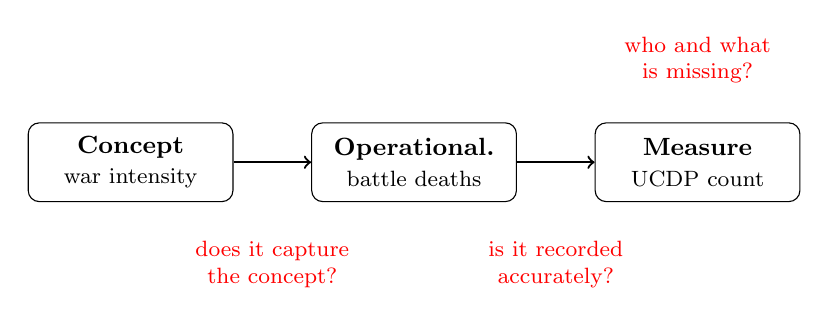
\begin{tikzpicture}[
  box/.style = {draw, rounded corners, minimum width = 2.6cm, minimum height = 1cm, align = center, font = \small},
  arr/.style = {->, thick}]
  \node[box] (c) at (0,0) {\textbf{Concept}\\{\footnotesize war intensity}};
  \node[box] (o) at (3.6,0) {\textbf{Operational.}\\{\footnotesize battle deaths}};
  \node[box] (m) at (7.2,0) {\textbf{Measure}\\{\footnotesize UCDP count}};
  \draw[arr] (c) -- (o);
  \draw[arr] (o) -- (m);
  \uncover<2->{
  \node[font = \footnotesize, text = red, align = center] at (1.8,-1.3) {does it capture\\the concept?};
  \node[font = \footnotesize, text = red, align = center] at (5.4,-1.3) {is it recorded\\accurately?};}
  \uncover<3->{
  \node[font = \footnotesize, text = red, align = center] at (7.2,1.3) {who and what\\is missing?};}
\end{tikzpicture}

\vspace{20pt}
\uncover<4->{{\small Deaths from famine and disease? Civilians? Wars below 25 deaths/year?}}

\end{frame}
% ----------------------------------------------------
\note{The picture for the whole first half. Every measurement problem today lives on one of these arrows.

\begin{itemize}
  \item First arrow, \textbf{validity}: battle deaths capture one dimension of intensity. A war that displaces a million people and kills few in combat is intense in any sense that matters, and invisible here.
  \item Second arrow, \textbf{recording}: deaths are counted from news reports, which are thinner in rural areas and in places journalists cannot reach.
  \item Above the measure, \textbf{coverage}: UCDP only counts conflicts above 25 battle-related deaths a year, and only direct deaths.
\end{itemize}

None of this makes the UCDP count bad. It makes it a specific measure of a specific thing, which is what every measure is.}

% ----------------------------------------------------
\begin{frame}
\frametitle{Your turn}
\centering

\begin{itemize}
  \item Your question is about some cause of \textbf{civil war outbreak}
  \vspace{8pt}
  \item Two concepts hiding in there:
  \begin{itemize}
    \item[1.] \textbf{Civil war}
    \item[2.] \textbf{Outbreak}
  \end{itemize}
  \vspace{8pt}
  \item How would you define each? How would you operationalize it?
\end{itemize}

\end{frame}
% ----------------------------------------------------
\note{Pairs, three minutes. ``Outbreak'' is the one nobody thinks about, and it is the interesting one.

Civil war: a threshold of deaths (1{,}000 a year is the classic one), a state as one party, an organised challenger. Each is a choice.

Outbreak: is it the first year above the threshold? The first violent event? What about a war that dips below 1{,}000 for two years and comes back: is that a new outbreak or the same war? Different datasets answer differently, and the list of ``outbreaks'' changes enough to change results.

Good place to say: \textbf{a huge share of published disagreement in some fields is really disagreement about coding rules}, not about the world.}

% ----------------------------------------------------
\begin{frame}
\frametitle{Why this is not a philosophy detour}
\centering

\vspace{10pt}
\begin{itemize}[<+->]
  \item A large share of good quantitative work \textit{is} better concepts and better measures
  \vspace{8pt}
  \item Especially in CSS: new data mostly means \textbf{new ways to measure old concepts}
  \begin{itemize}
    \item ideology from follow networks, wealth from phone records, state reach from road maps
  \end{itemize}
  \vspace{8pt}
  \item Today's paper is exactly this
\end{itemize}

\end{frame}
% ----------------------------------------------------
\note{Sharpen this for this cohort. Many of them think the contribution of computational work is the method. Much more often it is the measurement: a concept that was expensive or impossible to observe becomes cheap to observe.

All three examples in the sub-bullet are in the course: Barberá later today, Blumenstock from week 1, Müller-Crepon as the paper. In each case the contribution is ``we can now measure X'', and the whole paper stands or falls on whether the new measure means what they claim.}

% ====================================================
\section{Measuring the right stuff}
% ====================================================

% ----------------------------------------------------
\begin{frame}
\frametitle{Three measurement questions}
\centering

\vspace{10pt}
\begin{itemize}
  \item[1.] Are you measuring \textbf{what you think} you are measuring?
  \begin{itemize}
    \item proxies, latent variables, model outputs
  \end{itemize}
  \vspace{8pt}
  \item[2.] Who or what are you \textbf{not} measuring?
  \begin{itemize}
    \item missing data, selection
  \end{itemize}
  \vspace{8pt}
  \item[3.] At \textbf{which level}?
  \begin{itemize}
    \item the unit of analysis, again
  \end{itemize}
\end{itemize}

\end{frame}
% ----------------------------------------------------
\note{The map for the next hour. Most of the time goes on the first one, because that is where CSS work is most exposed.}

% ----------------------------------------------------
\begin{frame}
\frametitle{How was this number made?}
\centering

\begin{itemize}
  \item We usually look at a variable without asking how it was created
  \vspace{8pt}
  \item<2-> Look closer:
  \begin{itemize}
    \item<2-> survey wording
    \item<2-> coding rules (who decided what counts as a democracy?)
    \item<2-> raw material (news reports? experts? admin records? posts?)
  \end{itemize}
  \vspace{8pt}
  \item<3-> Above all: are there \textbf{biases related to your question}?
\end{itemize}

\end{frame}
% ----------------------------------------------------
\note{The third bullet is the one that matters. Every measure has error. The design question is whether the error is \textit{related to what you are studying}. Random noise costs you precision; error that correlates with your explanatory variable manufactures results.

That distinction will come back three times today: discrimination data, Obermeyer, and classifiers.}

% ----------------------------------------------------
\begin{frame}
\frametitle{Example: measuring discrimination}
\centering

\begin{itemize}
  \item Question: does discrimination of minorities hurt a country's economic performance?
  \vspace{6pt}
  \item<2-> You find a dataset scoring each minority's discrimination, 0 to 10
  \begin{itemize}
    \item<2-> {\small codebook: ``unequal access to state power, from active discrimination (incl.\ mass violence) to lack of access to key positions''}
  \end{itemize}
  \vspace{6pt}
  \item<3-> Coded by sending a questionnaire to 2--3 country experts
  \vspace{6pt}
  \item<4-> \textbf{Thoughts?}
\end{itemize}

\end{frame}
% ----------------------------------------------------
\note{Let them find the problems. Two usually come up:
\begin{itemize}
  \item The concept is \textit{political} exclusion, and the question is about economic performance. Is political exclusion the kind of discrimination that should affect the economy? Maybe, but it is a specific claim.
  \item Experts know how the economy is doing. If they rate discrimination partly by looking at how badly things are going, the measure is contaminated by the outcome.
\end{itemize}

The second is the dangerous one: the error is related to the question.}

% ----------------------------------------------------
\begin{frame}
\frametitle{Same data, different question}
\centering

\begin{itemize}
  \item Now: does \textbf{extreme} discrimination make violence against minorities more likely?
  \begin{itemize}
    \item violence from another dataset, coded from newspapers
  \end{itemize}
  \vspace{8pt}
  \item You find a \textbf{positive relationship}
  \vspace{8pt}
  \item<2-> Go back to the definition
  \vspace{8pt}
  \item<3-> And: comparing \textit{within} countries, or \textit{between} them?
\end{itemize}

\end{frame}
% ----------------------------------------------------
\note{The definition \textit{includes} mass violence at the top of the scale. So ``extreme discrimination predicts violence'' is partly ``violence predicts violence''. The relationship is built into the measure.

This happens constantly, and it is almost always invisible unless someone reads the codebook. It is the strongest argument for reading it.

Within versus between: experts in different countries may use the scale differently (one country's 6 is another's 4), which is fine for comparing a group over time within a country and a problem for comparing across countries. Leave that as a teaser; comparability comes back in the description section.}

% ----------------------------------------------------
\begin{frame}
\frametitle{Has democracy declined?}
\centering

\begin{itemize}
  \item Widespread claim: the world is going through \textbf{democratic backsliding}
  \vspace{8pt}
  \item Problem: how do we measure democracy?
  \vspace{8pt}
  \item Most global indices rely on \textbf{expert judgement}
\end{itemize}

\end{frame}
% ----------------------------------------------------
\note{The best measurement example in the course, because it is a live debate among serious people and the disagreement is almost entirely about measurement.

Ask for a show of hands first: has the world become less democratic in the last fifteen years? Almost everyone says yes. Keep that in mind for two slides from now.}

% ----------------------------------------------------
\begin{frame}[plain]
  \begin{tikzpicture}[remember picture, overlay]
    \node[at = (current page.center), yshift = 0cm] (cover) {%
      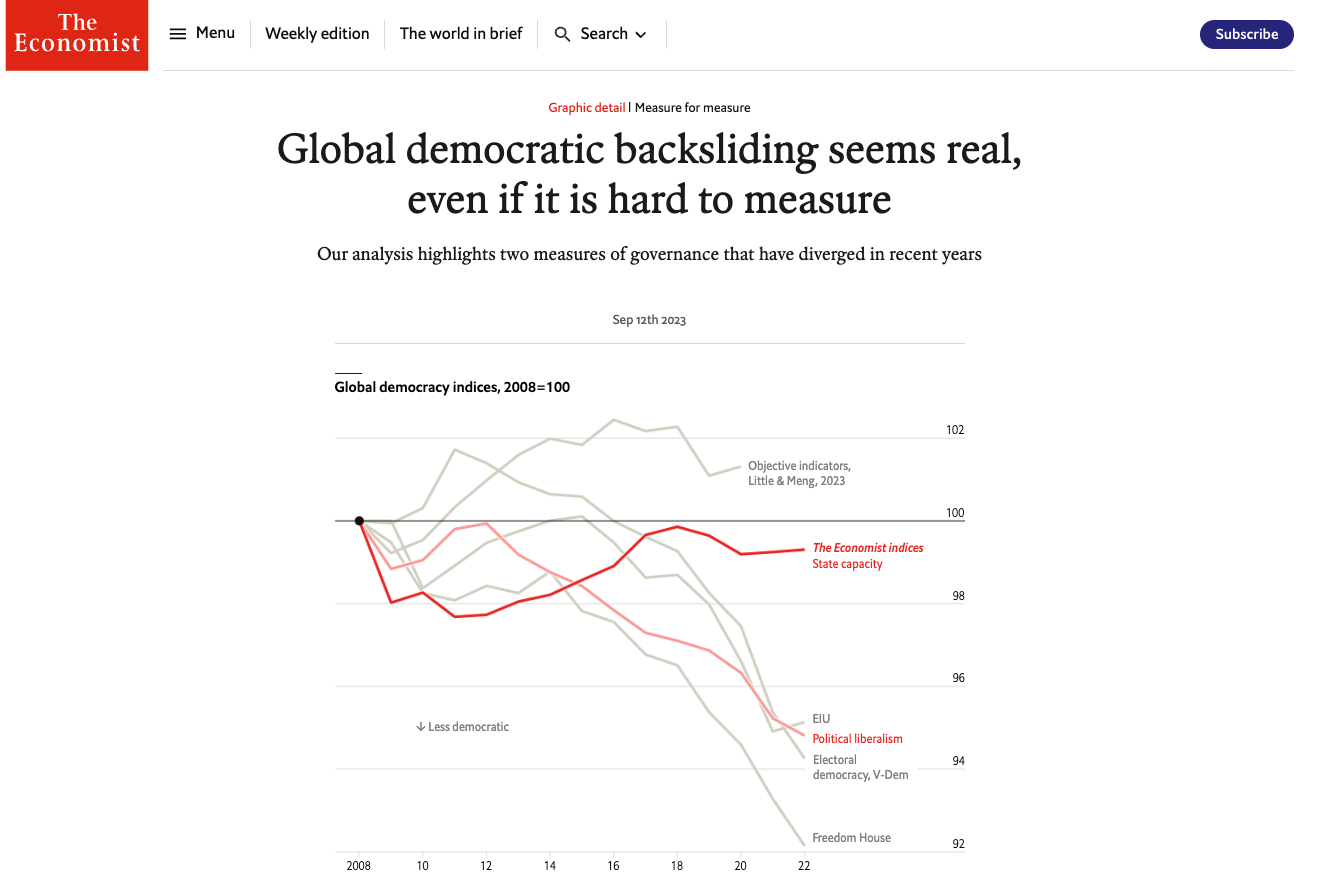
\includegraphics[keepaspectratio, width=\paperwidth, height=\paperheight]{../img/economist_backsliding}};
  \end{tikzpicture}
\end{frame}
% ----------------------------------------------------
\note{The Economist, 2023. Several indices, all normalised to 2008 = 100.

Point at the divergence: Freedom House, V-Dem and EIU go down clearly after 2015. The grey line at the top, ``objective indicators'', does not. Same world, same years, different conclusions.

Ask: which one is right? Wrong question. Better: what is each one measuring?}

% ----------------------------------------------------
\begin{frame}[plain]
  \begin{tikzpicture}[remember picture, overlay]
    \node[at = (current page.center), yshift = 0cm] (cover) {%
      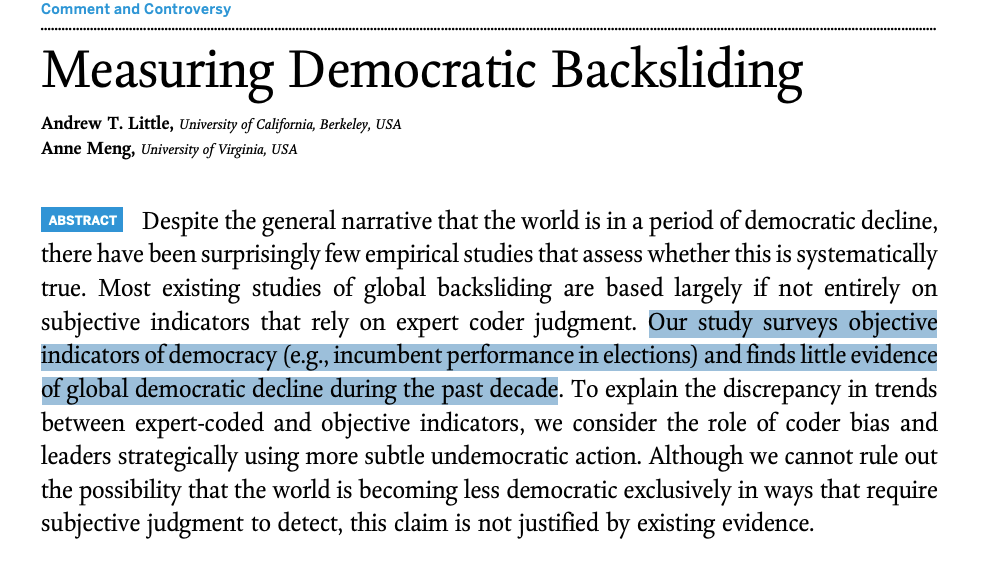
\includegraphics[keepaspectratio, width=\paperwidth, height=.8\paperheight]{../img/little_meng}};
  \end{tikzpicture}
\end{frame}
% ----------------------------------------------------
\note{Little \& Meng (2024, \textit{PS}): using objective indicators, such as whether incumbents lose elections, they find little evidence of global decline in the last decade.

Their two explanations for the gap are the interesting part: \textbf{coder bias} (experts are reading the same news and the same narrative), and \textbf{strategic autocrats} who backslide in subtle ways only a human can see. Notice they cannot rule out the second. The disagreement cannot be settled with more data of either kind.}

% ----------------------------------------------------
\begin{frame}
\frametitle{Two operationalizations of democracy}
\centering

\small
\begin{columns}[T]
\begin{column}{0.47\textwidth}
\centering \textbf{`Objective'}
\vspace{4pt}
\hrule
\vspace{6pt}
\begin{flushleft}
\footnotesize
Minimalist concept: contested elections\\[6pt]
e.g.\ Democracy \& Dictatorship:\\
1.\ elected executive\\
2.\ elected legislature\\
3.\ more than one party\\
4.\ alternation in power has happened\\[6pt]
\uncover<2->{\textbf{But}: incumbents losing elections is not so objective either (young, growing democracies)}
\end{flushleft}
\end{column}
\begin{column}{0.47\textwidth}
\centering \textbf{`Subjective'}
\vspace{4pt}
\hrule
\vspace{6pt}
\begin{flushleft}
\footnotesize
Maximalist concept: elections, plus rule of law, media, participation\ldots\\[6pt]
e.g.\ V-Dem: expert surveys, several coders per country, with measures of uncertainty\\[6pt]
\uncover<2->{\textbf{But}: autocrats are creative, and experts read the same newspapers}
\end{flushleft}
\end{column}
\end{columns}

\end{frame}
% ----------------------------------------------------
\note{The design lesson is on this slide. The two camps are not measuring the same concept badly and well; they are measuring \textbf{different concepts}.

A minimalist measure is replicable and blind to anything that does not show up in elections. A maximalist measure sees subtle erosion and depends on human judgement. Choosing between them is a theoretical decision, made before any data.

Botswana: the same party won every election from 1966 to 2024, so rule 4 coded it a dictatorship for decades, although most called it a democracy. The 2024 opposition win reclassified it after the fact. ``Objective'' rules are still choices.

Transfer: when two measures of ``the same thing'' disagree, first ask whether they measure the same concept.}

% ----------------------------------------------------
\begin{frame}
\frametitle{Proxies}
\centering

\begin{itemize}
  \item A \textbf{proxy} stands in for something you cannot observe
  \item Creative, useful, and always a bet. What could bias these?
  \vspace{6pt}
  \begin{itemize}
    \item<2-> Economic development $\leftarrow$ night-time lights from satellites
    \item<3-> Household wealth $\leftarrow$ owning a TV
    \item<4-> Emigration (early 20th c.\ Spain) $\leftarrow$ missing men in the census
  \end{itemize}
\end{itemize}

\end{frame}
% ----------------------------------------------------
\note{Take one or two per item, fast. For each, the question is not ``is it a good proxy'' but ``when does it break, and is the breakage related to my question?''

\begin{itemize}
  \item Night lights: saturate in cities, miss agriculture, and track electrification policy as much as income.
  \item TV: tracks electrification and fashion, and stops discriminating once everyone has one.
  \item Missing men: also war deaths, seasonal work, under-registration.
\end{itemize}

Next slide: a proxy whose breakage was directly related to the question, with real consequences.}

% ----------------------------------------------------
\begin{frame}
\frametitle{A proxy that encoded the wrong thing}
\centering

\begin{itemize}
  \item US hospitals used an algorithm to decide who gets \textbf{extra care}
  \begin{itemize}
    \item algorithms like this reach $\sim$200 million people a year in the US
  \end{itemize}
  \vspace{6pt}
  \item<2-> Target: patients with the greatest \textbf{health need}
  \item<2-> What it actually used as a proxy: \textbf{healthcare cost}
  \item<2-> (The model was set to predict future healthcare costs, and so its finding could be interpreted to foresee healthcare needs)
  \vspace{6pt}
  \item<3-> What could go wrong?
\end{itemize}

\vspace{6pt}
\uncover<2->{{\footnotesize \asher{Obermeyer, Powers, Vogeli \& Mullainathan (2019), \textit{Science} 366(6464).}}}

% TODO: source the two-panel figure (chronic conditions vs. risk score, and cost vs. risk score, by race), save as ../img/obermeyer_bias.png
\end{frame}
% ----------------------------------------------------
\note{Build it slowly and make them get to the answer. The algorithm was accurate: it predicted cost well. Cost looks like a sensible proxy for need, because sicker people cost more.

The third bullet is the one to pause on. Most students assume that leaving race out makes a model fair. Ask them to hold that thought.

Take answers to the last bullet before turning the page. Someone usually gets it: less is spent on some patients for the same level of illness.}

% ----------------------------------------------------
\begin{frame}
\frametitle{Obermeyer et al.: what went wrong}
\centering

\begin{itemize}[<+->]
  \item People with better resources could spend more even if they had the exact same illness
  \item They did not include race in the models, deliberately so as not to discriminate
  \item But at equal illness, \textbf{less was spent} on Black patients
  \begin{itemize}
    \item unequal access to care, not less need
  \end{itemize}
  \vspace{8pt}
  \item So at the same risk score, Black patients were \textbf{considerably sicker}
  \vspace{8pt}
  \item Measuring need directly would have raised the share of Black patients flagged from \textbf{18\% to 47\%}
\end{itemize}

\vspace{12pt}
\uncover<4->{\centering The proxy was accurate. \colorbox{yellow}{It was accurate about the wrong thing.}}

\end{frame}
% ----------------------------------------------------
\note{Pure construct validity, and no statistics needed to see it.

Spending reflects need \textit{and} access, and access differs by race. A proxy built on spending inherits that inequality, and an accurate model faithfully reproduces it.

Race-blindness did not help because the bias was in the \textbf{outcome variable}, not the inputs.

Paper figures: 17.7\% to 46.5\%. The fix was a measurement fix, not a modelling one: change the label from cost to a direct measure of health.

Same structure: engagement for interest, arrests for crime (last week's re-offenders), clicks for preference.}

% ====================================================
\section{Latent variables and model outputs}
% ====================================================

% ----------------------------------------------------
\begin{frame}
\frametitle{Latent variables}
\centering

\begin{itemize}
  \item Some concepts cannot be observed directly, at all
  \begin{itemize}
    \item ideology, trust, state capacity, polarization
  \end{itemize}
  \vspace{8pt}
  \item Instead: \textbf{infer} them from several things you \textit{can} observe (i.e. from their traces)
  \vspace{8pt}
  \item<2-> Compare classic strategies for, e.g., party positions:
  \begin{itemize}
    \item<2-> expert surveys
    \item<2-> coding texts (manifestos, speeches)
    \item<2-> roll-call votes (\textbf{latent variable approach})
  \end{itemize}
  \item<3-> Each captures a slightly different concept
\end{itemize}

\end{frame}
% ----------------------------------------------------
\note{The idea without the statistics: if a concept is real, it should leave traces in several places, and you can triangulate from the traces back to the concept.

The three strategies for party positions are worth a sentence each, because they illustrate the last bullet: experts measure reputation, manifestos measure what parties \textit{say}, roll calls measure what legislators \textit{do} under party discipline. All of them are ``ideology''.}

% ----------------------------------------------------
\begin{frame}
\frametitle{Example: ideology on Twitter}
\centering

\begin{itemize}
  \item Do left- and right-wing users behave differently online?
  \vspace{6pt}
  \item The outcome is easy: content, frequency, networks
  \vspace{6pt}
  \item \textbf{But how do you measure ideology?}
  \begin{itemize}
    \item<2-> only politicians, where you know it? \asher{(selection)}
    \item<3-> link survey responses to accounts, with consent? \asher{(cost, non-response)}
    \item<4-> \textbf{infer it from behaviour}? (example from Barberá 2015, \textit{Pol Analysis})
  \end{itemize}
\end{itemize}

\end{frame}
% ----------------------------------------------------
\note{Incomplete, from last week's ten characteristics: the variable you need is not in the data. These are the three ways out, and each one has a price. The third is the typical CSS answer, and it is the one where measurement becomes a model.}

% ----------------------------------------------------
\begin{frame}[plain]
  \begin{tikzpicture}[remember picture, overlay]
    \node[at = (current page.center), yshift = 0cm] (cover) {%
      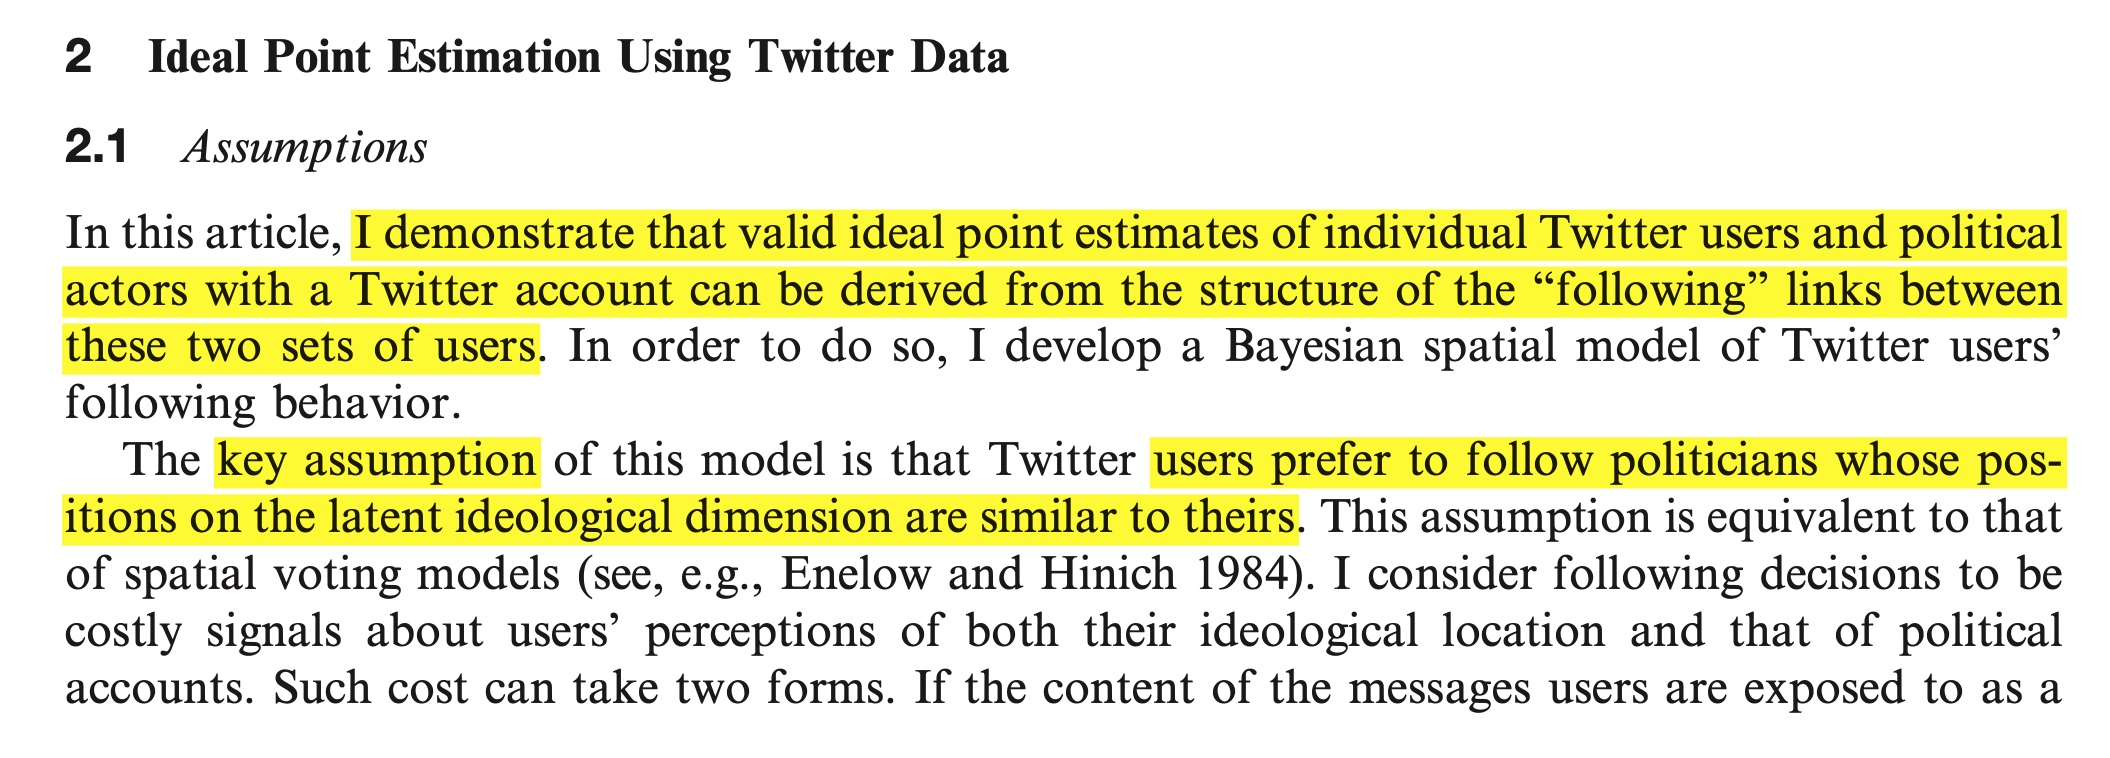
\includegraphics[keepaspectratio, width=.95\paperwidth, height=\paperheight]{../img/barbera_tw2}};
  \end{tikzpicture}
\end{frame}
% ----------------------------------------------------
\note{Barberá (2015), \textit{Political Analysis}. Ideology inferred from \textbf{who you follow}.

Read the highlighted assumption aloud: users prefer to follow politicians close to them ideologically. That is the whole measure. Everything else is estimation.

Ask: when would that assumption fail? Answers: journalists follow everyone; people hate-follow; people follow the government for information. The measure is as good as the assumption, and the assumption is a theory about behaviour.}

% ----------------------------------------------------
\begin{frame}[plain]
  \begin{tikzpicture}[remember picture, overlay]
    \node[at = (current page.center), yshift = 0cm] (cover) {%
      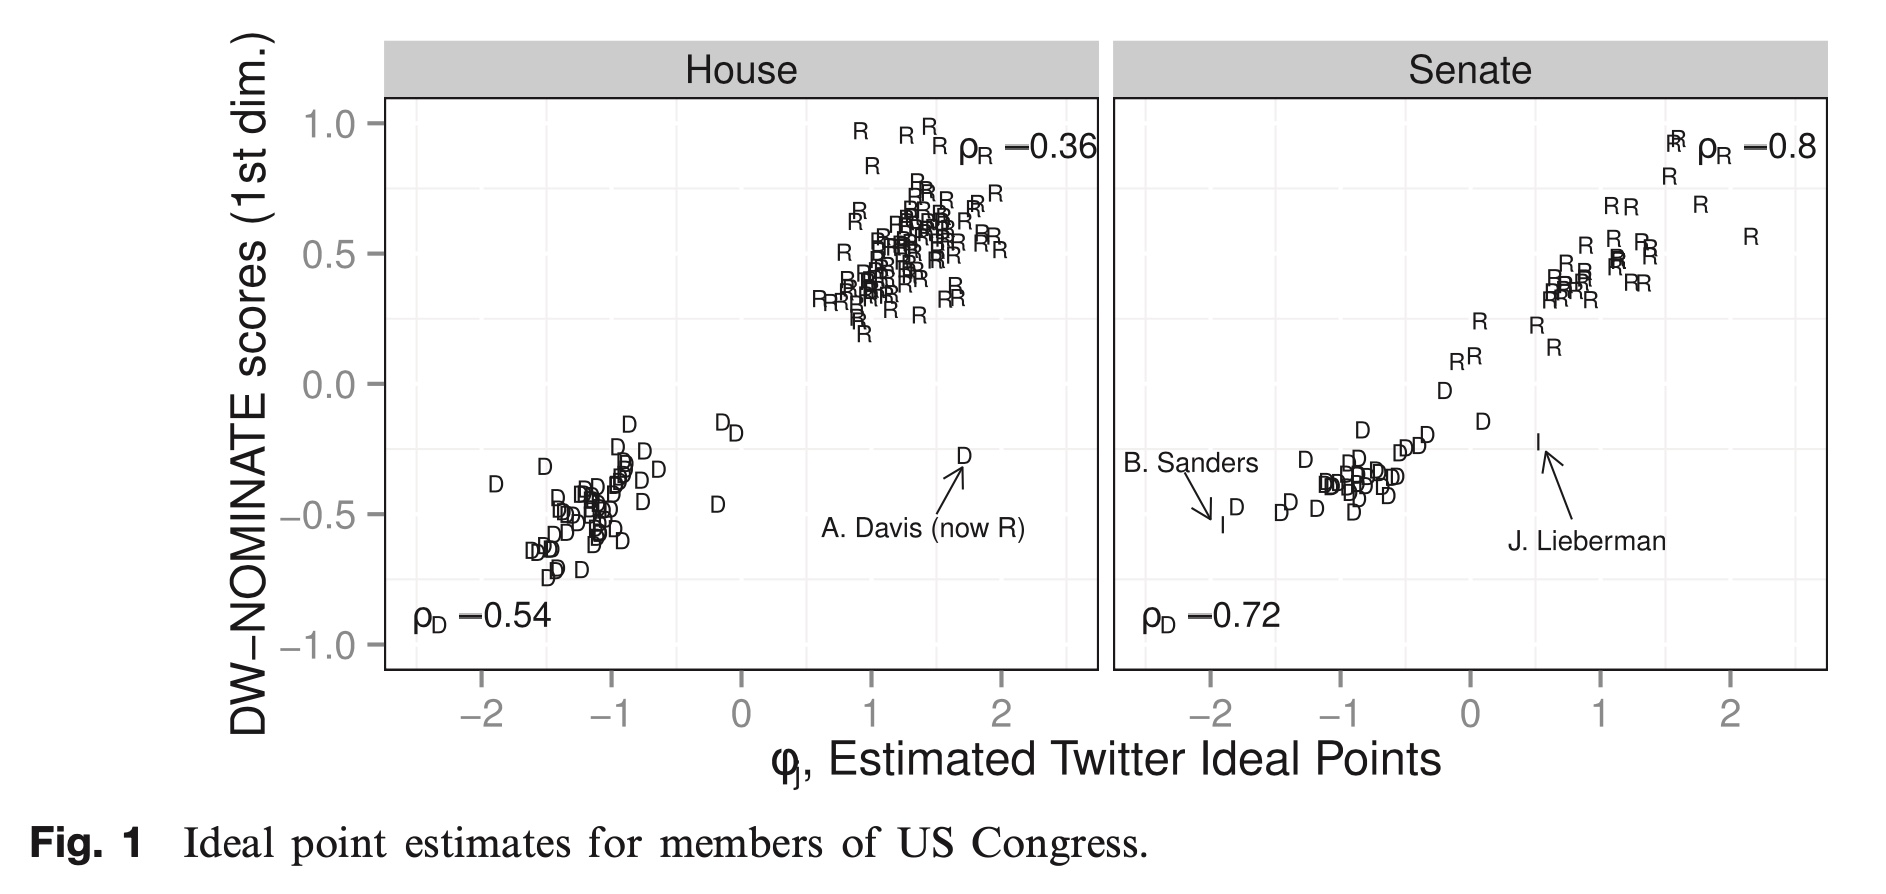
\includegraphics[keepaspectratio, width=.95\paperwidth, height=\paperheight]{../img/barbera_tw3}};
  \end{tikzpicture}
\end{frame}
% ----------------------------------------------------
\note{Validation, step one. For members of Congress we already know ideology from roll-call votes (DW-NOMINATE). Plot the Twitter estimate against it.

It separates the parties perfectly, and within parties it is correlated, more strongly in the Senate. The outliers are informative: Sanders and Lieberman are where you would expect.

The key design point: the measure is checked against something \textbf{built from completely different data}.}

% ----------------------------------------------------
\begin{frame}[plain]
  \begin{tikzpicture}[remember picture, overlay]
    \node[at = (current page.center), yshift = 0cm] (cover) {%
      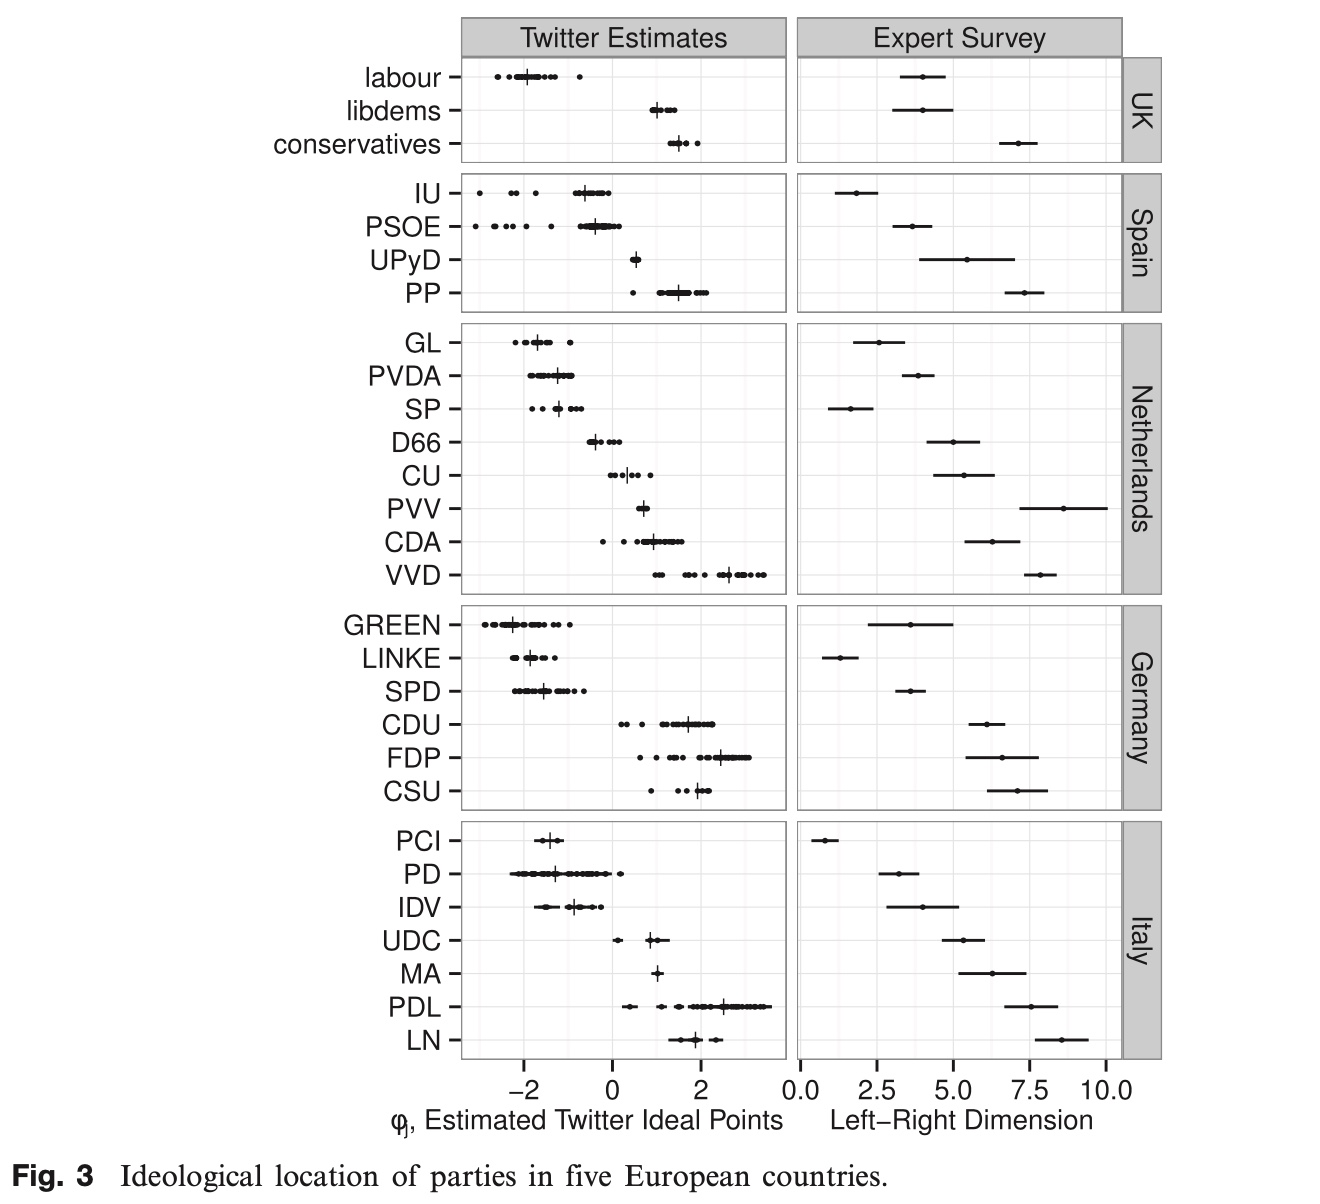
\includegraphics[keepaspectratio, width=\paperwidth, height=.95\paperheight]{../img/barbera_tw4}};
  \end{tikzpicture}
\end{frame}
% ----------------------------------------------------
\note{Step two: parties in five European countries against expert surveys. The ordering broadly matches. Point at Spain: IU, PSOE, UPyD, PP in the expected order.

Also point at where it does not match perfectly (e.g.\ PVV in the Netherlands). Validation is not a pass/fail stamp; it tells you where the measure is trustworthy and where it is not.

And note the gap nobody can close from this slide: validating on politicians does not prove it works on ordinary users. The paper also checks users who state their preferences publicly and users matched to party registration records. That is a third, separate check, aimed exactly at the population they care about.}

% ----------------------------------------------------
\begin{frame}
\frametitle{When your variable is a model's output}
\centering

\begin{itemize}
  \item Increasingly common: a variable that is the \textbf{prediction of a model}
  \begin{itemize}
    \item sentiment, toxicity, topic, stance, ideology
    \item inferred gender, age, location
    \item labels produced by an LLM
  \end{itemize}
  \vspace{8pt}
  \item<2-> The measurement question does not go away. It gets \textbf{harder}
  \vspace{8pt}
  \item<3-> Because the error is almost never random
\end{itemize}

\end{frame}
% ----------------------------------------------------
\note{The new block, and the one most directly relevant to what this cohort will actually do. Many of their theses will have a variable that came out of a classifier, and increasingly out of a prompt to a language model.

The seductive thing is that the output looks like data: a clean column of numbers. It is a measurement, made by an instrument whose error you usually have not characterised.

Next slide: why ``not random'' is the whole problem.}

% ----------------------------------------------------
\begin{frame}
\frametitle{Non-random errors in CSS}
\centering

\vspace{5pt}
\begin{itemize}[<+->]
  \item A toxicity classifier flags more posts as toxic when written in some dialects
  \begin{itemize}
    \item ``group X is more toxic'' is partly ``the classifier reads group X badly''
  \end{itemize}
  \vspace{8pt}
  \item A sentiment model trained on English, applied to Spanish and Catalan
  \begin{itemize}
    \item the comparison across languages is partly a comparison of accuracy
  \end{itemize}
  \vspace{8pt}
  \item An LLM labels posts, then the model is updated
  \begin{itemize}
    \item drift, last week: the instrument changed underneath you
  \end{itemize}
  \item See Knox et al (2022), `Testing Causal Theories with
Learned Proxies' for more
\end{itemize}



\end{frame}
% ----------------------------------------------------
\note{Three concrete cases. In each, the error is \textbf{correlated with the thing you want to compare}, so it does not just add noise; it produces differences that are not there.

The first is documented: Sap et al.\ (2019) showed that toxicity classifiers flagged tweets in African American English as offensive much more often. Any study comparing toxicity across groups with such a tool is measuring the tool.

The third is worth a minute. If you label a corpus with a hosted model, the model can change without notice. Record the version, and keep a hand-coded sample so that you can check.

Knox, Lucas \& Cho (2022, \textit{ARPS}) is the reference if anyone wants the formal version. The intuition is all we need.}

% ----------------------------------------------------
\begin{frame}
\frametitle{The rule: validate, always}
\centering

\vspace{5pt}
\begin{itemize}[<+->]
  \item There is no automatic method that is valid everywhere
  \begin{itemize}
    \item the ``no free lunch''
  \end{itemize}
  \vspace{6pt}
  \item Validate against something \textbf{external}:
  \begin{itemize}
    \item a hand-coded sample (by humans, blind to the model)
    \item a known group (politicians, registered party members)
    \item another measure built from different data
  \end{itemize}
  \vspace{6pt}
  \item And validate \textbf{in the population you will use it on}
\end{itemize}

\vspace{8pt}
\uncover<3->{{\footnotesize \asher{Grimmer, Roberts \& Stewart (2022), \textit{Text as Data}.}}}

\end{frame}
% ----------------------------------------------------
\note{The practical rule for their essays, and it is worth being prescriptive: \textbf{if your design has a variable produced by a model, the design has to include a validation step.} Not optional, not a robustness check in an appendix.

The last bullet is where most validations quietly fail: a classifier validated on news articles and used on tweets, or an ideology measure validated on politicians and used on teenagers. Barberá did the extra check for exactly this reason.

This is a design decision, not a statistical one: it has to be planned before the data is collected, because you need to budget the hand-coding.}

% ====================================================
\section{Who is missing, and at which level}
% ====================================================

% ----------------------------------------------------
\begin{frame}
\frametitle{Missing data}
\centering

\begin{itemize}
  \item Almost always more important than it looks
  \vspace{6pt}
  \item<2->[1.] Missing \textbf{completely at random} (MCAR)
  \begin{itemize}
    \item<2-> no pattern at all. Rare
  \end{itemize}
  \item<3->[2.] Missing \textbf{at random} (MAR)
  \begin{itemize}
    \item<3-> depends only on things you \textit{observe}, so you can adjust for it
  \end{itemize}
  \item<4->[3.] Missing \textbf{not at random} (MNAR)
  \begin{itemize}
    \item<4-> missingness is related to the thing you are studying
  \end{itemize}
\end{itemize}

\end{frame}
% ----------------------------------------------------
\note{Three categories, and they only need to remember the logic, not the names. The question is always the same as before: is the missingness related to what you are studying?}

% ----------------------------------------------------
\begin{frame}
\frametitle{Missing data: example}
\centering

\begin{itemize}
  \item \textbf{Our question:} Does some habit reduce post-surgery recovery time?
  \item \textbf{How we get the data:} Forms filled in at hospital check-in, some are missing. Why?
  \vspace{8pt}
  \item[1.] A random batch of forms got lost $\Rightarrow$ MCAR \asher{\small (although\ldots)}
  \vspace{4pt}
  \item[2.] One (recorded) admin worker always forgets to ask $\Rightarrow$ MAR \asher{\small (although\ldots)}
  \vspace{4pt}
  \item[3.] Emergencies do not fill in forms $\Rightarrow$ MNAR
\end{itemize}

\end{frame}
% ----------------------------------------------------
\note{The ``although'' tags are the good part. Ask what could make each one worse than it looks.

\begin{itemize}
  \item Lost forms: lost on which day? If it was a weekend batch, and weekend patients differ, it is not completely random.
  \item The forgetful admin: works which shift? Night-shift patients are more often emergencies.
  \item Emergencies are exactly the sickest patients, with the longest recovery. Dropping them changes the answer.
\end{itemize}

Callback to Challenger and the bombers: the observations that are missing are often the informative ones.}

% ----------------------------------------------------
\begin{frame}
\frametitle{Selection, again}
\centering

\begin{itemize}
  \item Sometimes the sample was designed with a bias
  \begin{itemize}
    \item an online survey and people over 65
  \end{itemize}
  \vspace{8pt}
  \item<2-> Harder to see: an \textbf{invisible filter} decides who is in the data
  \begin{itemize}
    \item<2-> who consents to share their feed with researchers
    \item<2-> who posts at all
  \end{itemize}
  \vspace{8pt}
  \item<3-> Remember the Xbox poll: the skew is fine \textbf{only if you know it and can correct for it}
\end{itemize}

\end{frame}
% ----------------------------------------------------
\note{Selection as a measurement problem: your variable is measured only for units that passed a filter.

The last bullet is a deliberate correction. The Xbox example last week risks being read as ``non-representative samples are fine''. The lesson was the opposite: they were fine \textit{because} the researchers knew exactly how the sample was skewed and had external data to correct it. Without that, the skew is fatal at any sample size.

Consent-based platform studies are next week's paper: who agreed to take part in Guess et al., and does that matter? Plant the question.}

% ----------------------------------------------------
\begin{frame}
\frametitle{At which level?}
\centering

\begin{itemize}
  \item The unit of analysis, again
  \vspace{6pt}
  \item Not all variables live at the same level
  \begin{itemize}
    \item individual data, household income; tweet data, user ideology
  \end{itemize}
  \vspace{6pt}
  \item<2-> Choose the level that matches the \textbf{theory and mechanism}
  \begin{itemize}
    \item<2-> e.g. wealth and voting in the US, state-level vs individual-level
  \end{itemize}
  \vspace{6pt}
  \item<3-> Measuring at the wrong level can change the answer
\end{itemize}

\end{frame}
% ----------------------------------------------------
\note{Short, because week 1 covered it. Two points only.

First, variables at different levels are normal and you have to decide where they meet: is the post the unit, or the user? A user with 10{,}000 posts dominates a post-level analysis.

Second, the ecological point in one line: a relationship between regions does not have to hold between individuals. Richer US states vote more Democratic; richer individuals within states vote more Republican. Same data, opposite answers at two levels.}

% ----------------------------------------------------
\begin{frame}
\frametitle{First half in four lines}
\centering

\vspace{15pt}
\begin{itemize}
  \item Concept $\rightarrow$ operationalization $\rightarrow$ measure
  \vspace{6pt}
  \item Error is fine. \textbf{Error related to your question} is not
  \vspace{6pt}
  \item Model outputs are measures. Validate them
  \vspace{6pt}
  \item Ask who is missing, and at which level
\end{itemize}

\vspace{15pt}
Questions?

\end{frame}
% ----------------------------------------------------
\note{Four lines. Break here, ten minutes.

After the break: description. Everything in the first half becomes concrete, because description is the goal where measurement is all you have.}

% ====================================================
\section{Description as a goal}
% ====================================================

% ----------------------------------------------------
\begin{frame}
\frametitle{Is description useful?}
\centering

\begin{itemize}[<+->]
  \item Not every question needs a \textit{why}
  \begin{itemize}
    \item has political violence increased? how segregated are friendships? how many people are 3 steps away?
  \end{itemize}
  \vspace{8pt}
  \item Description is not the consolation prize for failing to find a cause
  \vspace{8pt}
  \item It has its own design requirements:
  \begin{itemize}
    \item a clear \textbf{population}
    \item a defensible \textbf{denominator}
    \item \textbf{coverage} and \textbf{comparability} across units and time
  \end{itemize}
\end{itemize}

\end{frame}
% ----------------------------------------------------
\note{Make the argument properly, because students arrive thinking description is what you do before the real analysis.

Description is the first goal of the triad for a reason. Every causal question presupposes a description: you cannot explain the rise of political violence before establishing that it rose. And many of the most influential pieces of social science are descriptive.

The three requirements are the checklist for the rest of this section. Each example that follows fails or succeeds on one of them.}

% ----------------------------------------------------
\begin{frame}
\frametitle{Before anything: look at the data}
\centering

\begin{itemize}
  \item These are \textbf{real-world observations}. Plot your main variables
  \vspace{6pt}
  \item Is the distribution what the theory expects?
  \begin{itemize}
    \item bimodal where you expected one peak?
    \item a spike at 0, or at 99?
    \item a jump in one year?
  \end{itemize}
  \vspace{6pt}
  \item<2-> The shape can say something about the \textbf{mechanism}
  \begin{itemize}
    \item<2-> the effect of income in a very unequal vs.\ a very equal society
  \end{itemize}
\end{itemize}

\end{frame}
% ----------------------------------------------------
\note{Practical advice, and worth being blunt: plot every main variable before any analysis. It catches the 98 = refused problem from the Afrobarometer codebook last week, and it catches drift (a jump the year the platform changed).

The last bullet is a nice one to ask about: if income is bimodal, ``the average effect of income'' may be describing a difference between two groups rather than a gradient.}

% ----------------------------------------------------
\begin{frame}
\frametitle{A descriptive theory}
\centering

\vspace{10pt}
\textit{I read somewhere that everybody on this planet is separated by only six other people. Six degrees of separation. Between us and everybody else on this planet. The president of the United States. A gondolier in Venice.}\\\vspace{6pt}{\small John Guare, \textit{Six Degrees of Separation}}

\vspace{20pt}
\begin{itemize}
  \item A claim with no \textit{why} in it. Can we check it?
\end{itemize}

\end{frame}
% ----------------------------------------------------
\note{A purely descriptive claim that people have wondered about for a century (Milgram's letters in the 1960s). Ask how you would check it. Then show what Facebook did.}

% ----------------------------------------------------
\begin{frame}
\frametitle{Facebook: 3.57 degrees}
\centering

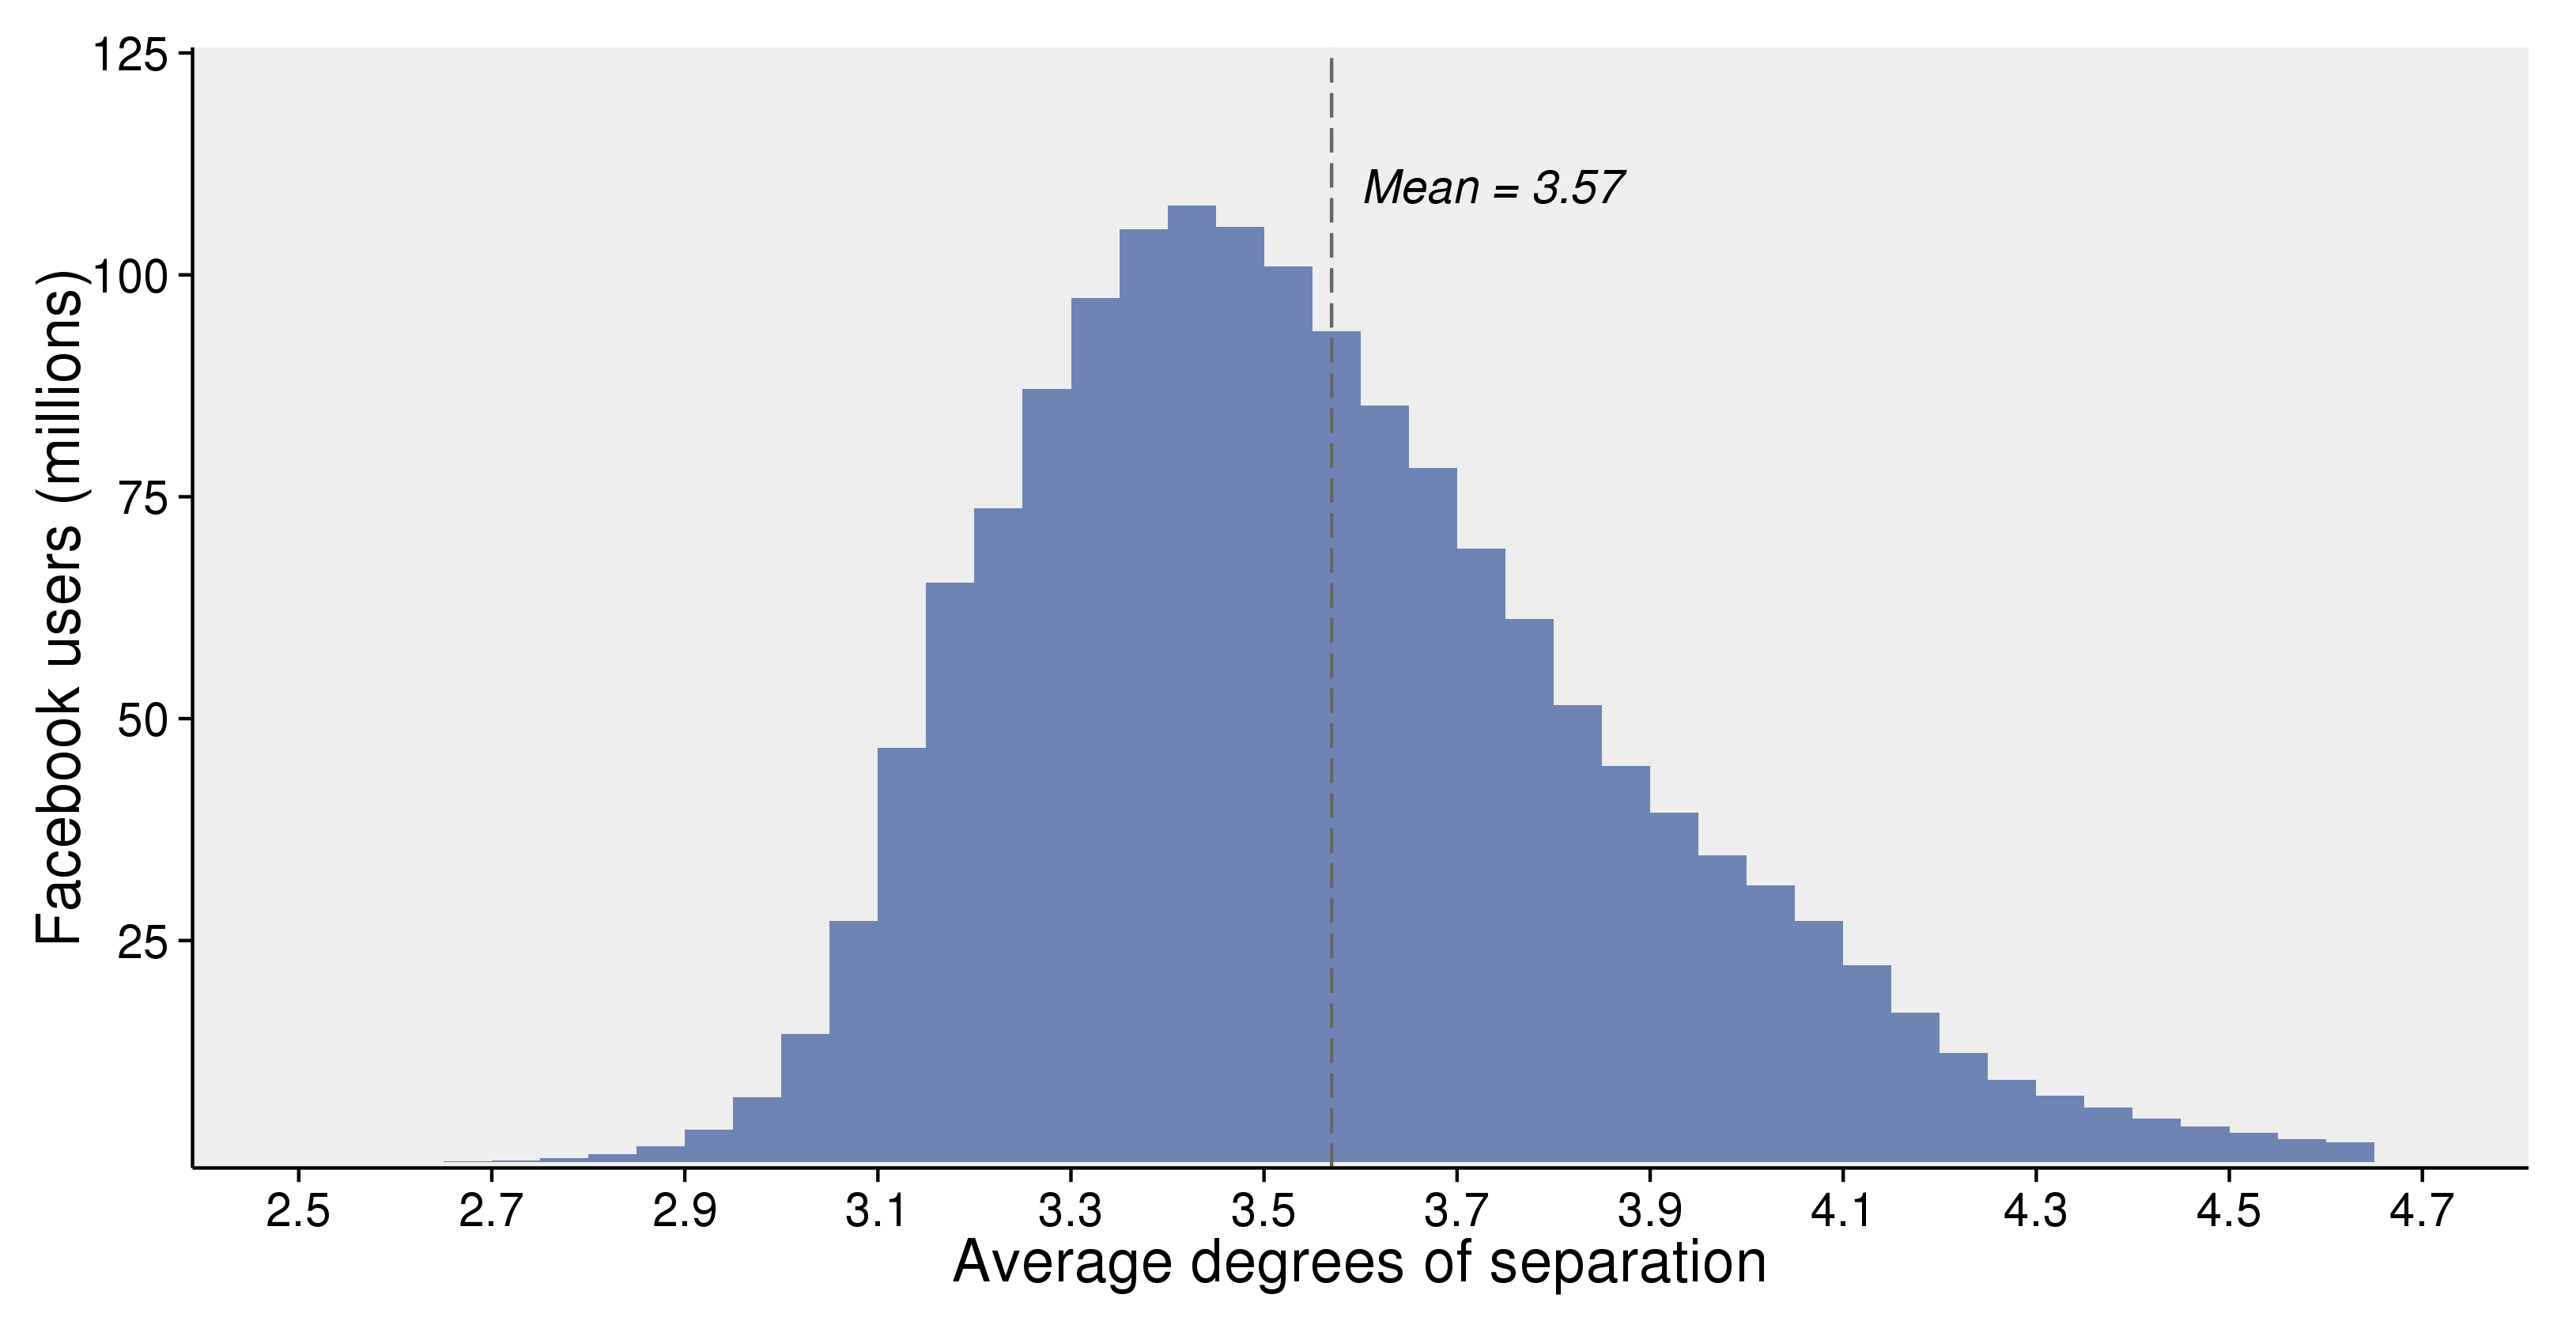
\includegraphics[keepaspectratio, width=\textwidth, height=0.6\paperheight]{../img/facebook_separation}

{\footnotesize Average degrees of separation between Facebook users, 2016.}

\end{frame}
% ----------------------------------------------------
\note{Facebook Research (2016): average separation of 3.57 among 1.6 billion users.

Now run the checklist:
\begin{itemize}
  \item \textbf{Population}: Facebook users, not ``everybody on this planet''. Who is not on Facebook? The gondolier maybe; billions of people certainly.
  \item \textbf{Operationalization}: is a Facebook friend the same as knowing someone? Much looser, which pushes the number down.
  \item \textbf{Comparability}: Milgram's six and Facebook's 3.57 measure different things, so the drop is not evidence that the world got smaller.
\end{itemize}

Descriptively impressive, and the answer to a slightly different question than the one Guare asked.}

% ----------------------------------------------------
\begin{frame}[plain]
  \begin{tikzpicture}[remember picture, overlay]
    \node[at = (current page.center), yshift = 0cm] (cover) {%
      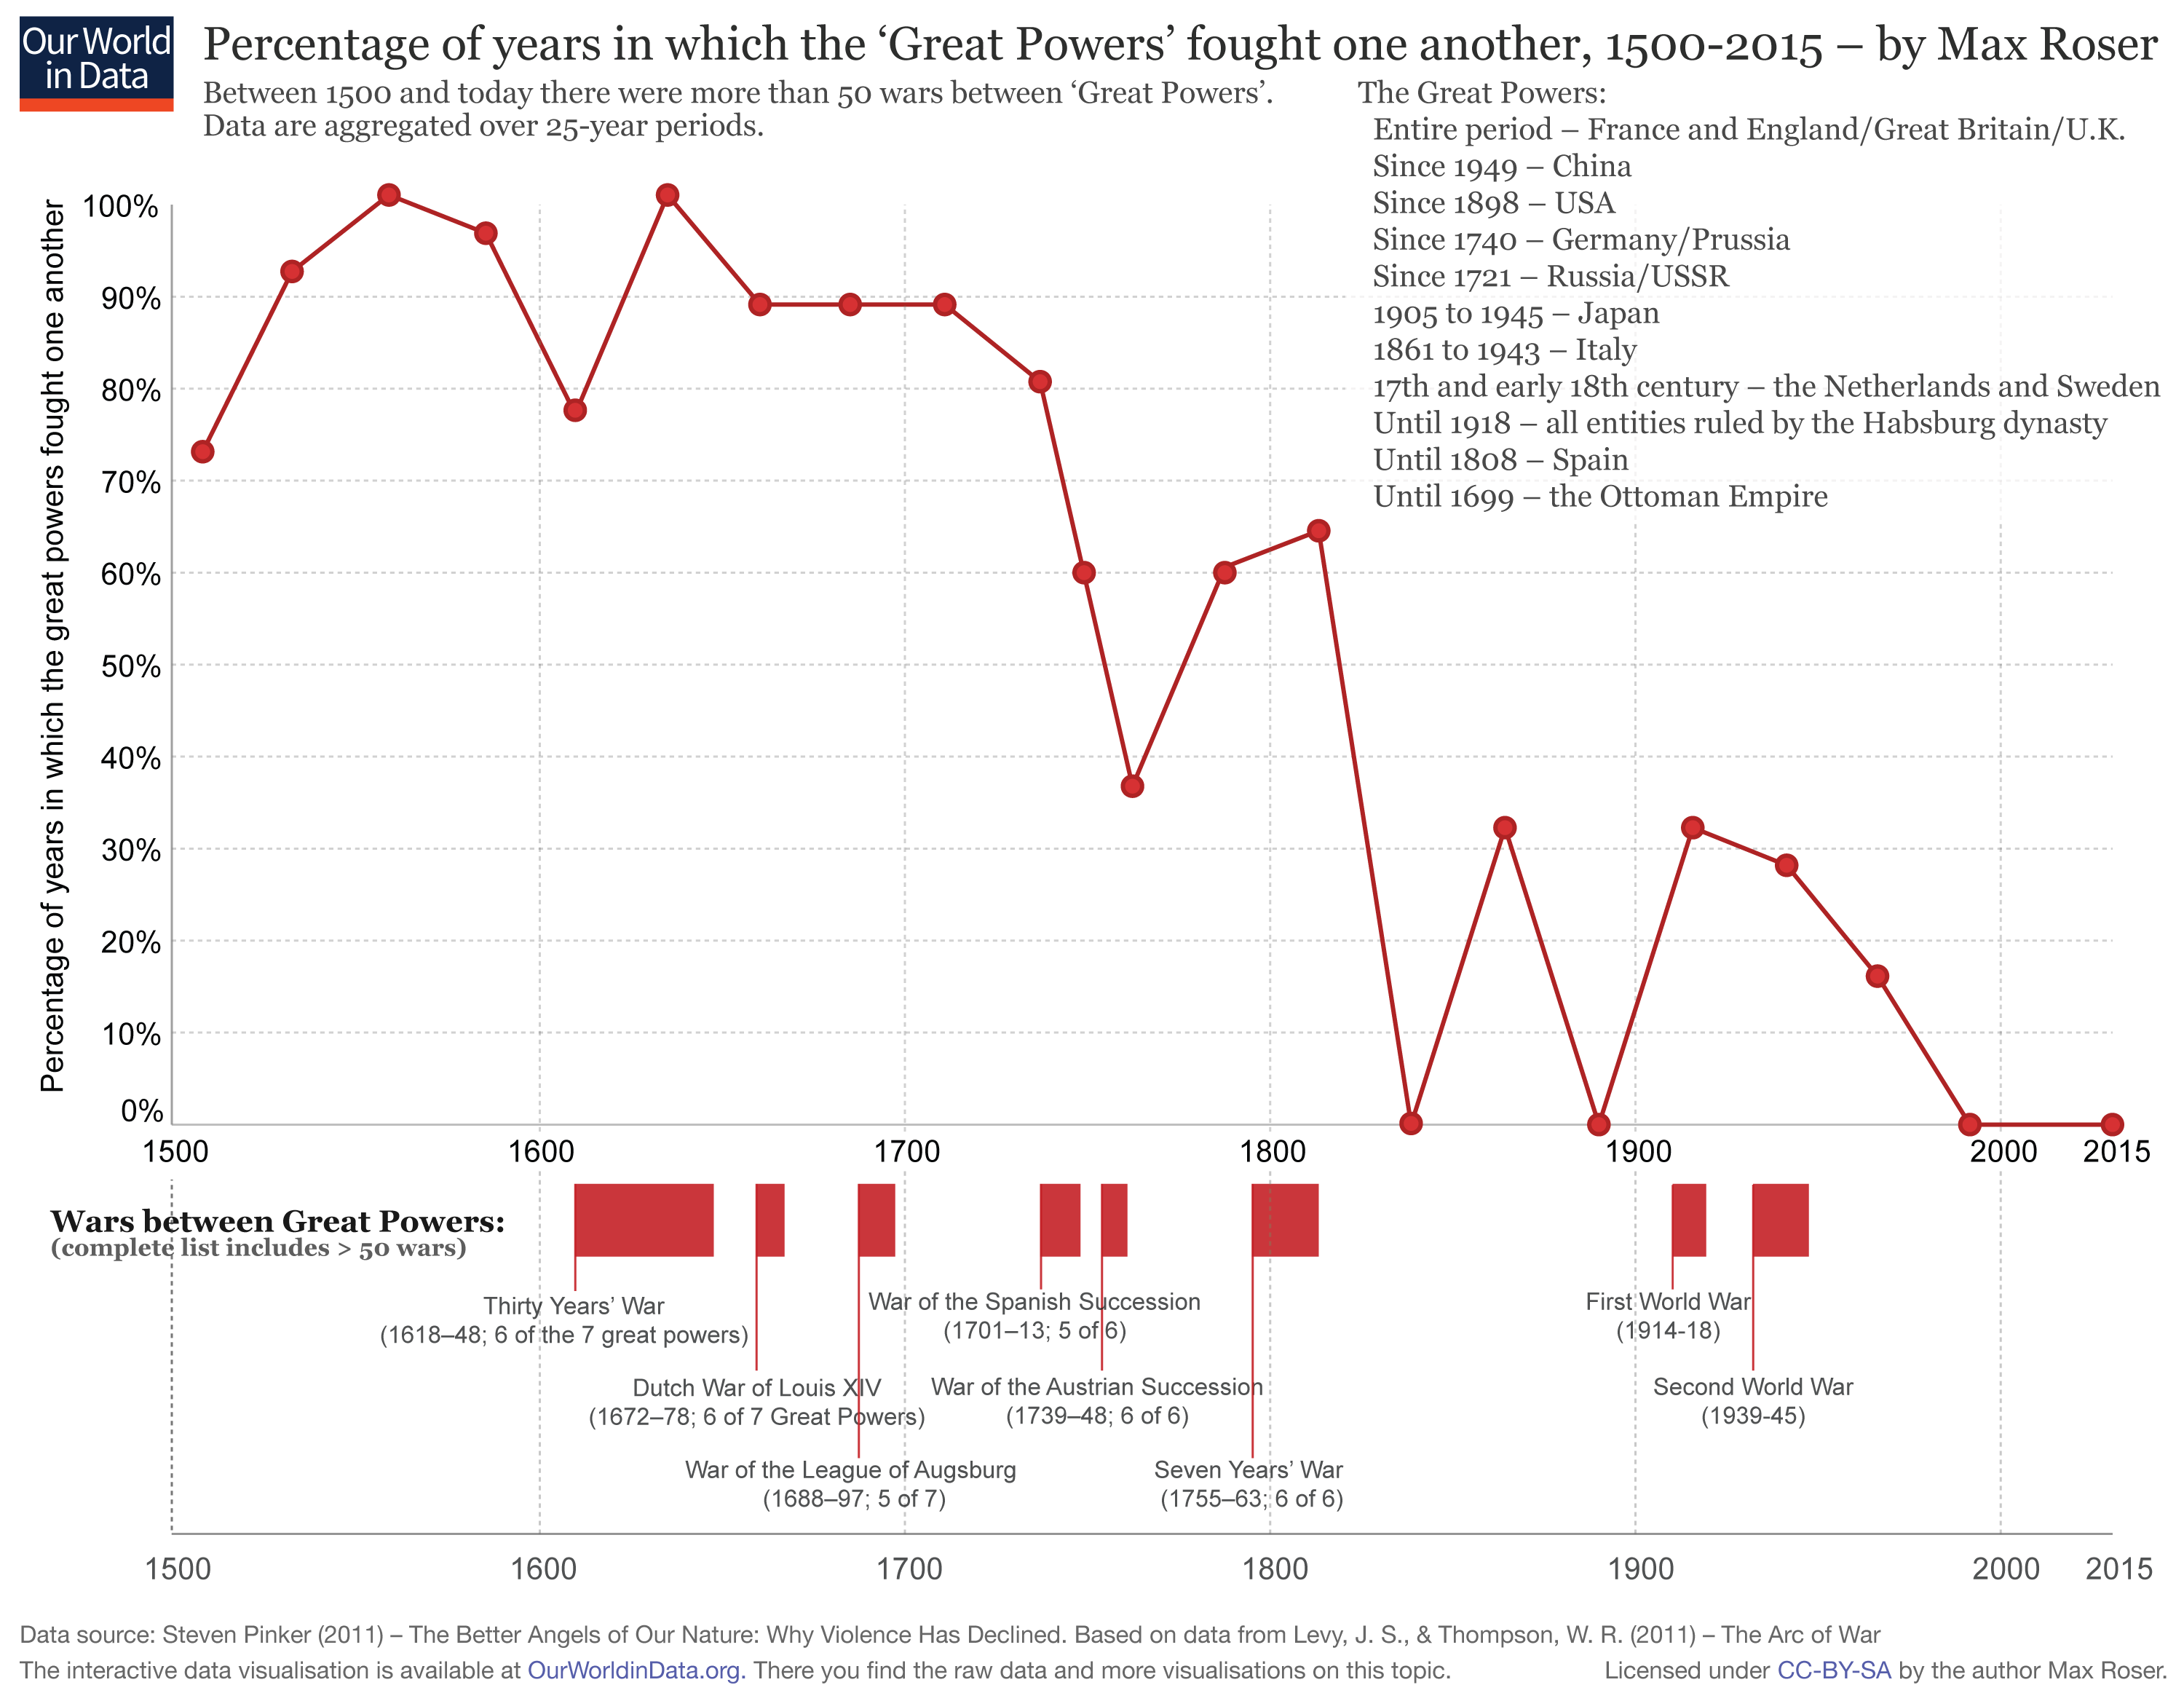
\includegraphics[keepaspectratio, width=\paperwidth, height=.95\paperheight]{../img/declineofwar}};
  \end{tikzpicture}
\end{frame}
% ----------------------------------------------------
\note{Another descriptive claim with a big literature: war has declined (Pinker). This version: share of years in which the great powers fought each other. A dramatic decline.

Ask what the operationalization is doing. It only counts wars \textit{between great powers}, and the list of great powers is itself a coding decision that changes over time.}

% ----------------------------------------------------
\begin{frame}[plain]
  \begin{tikzpicture}[remember picture, overlay]
    \node[at = (current page.center), yshift = 0cm] (cover) {%
      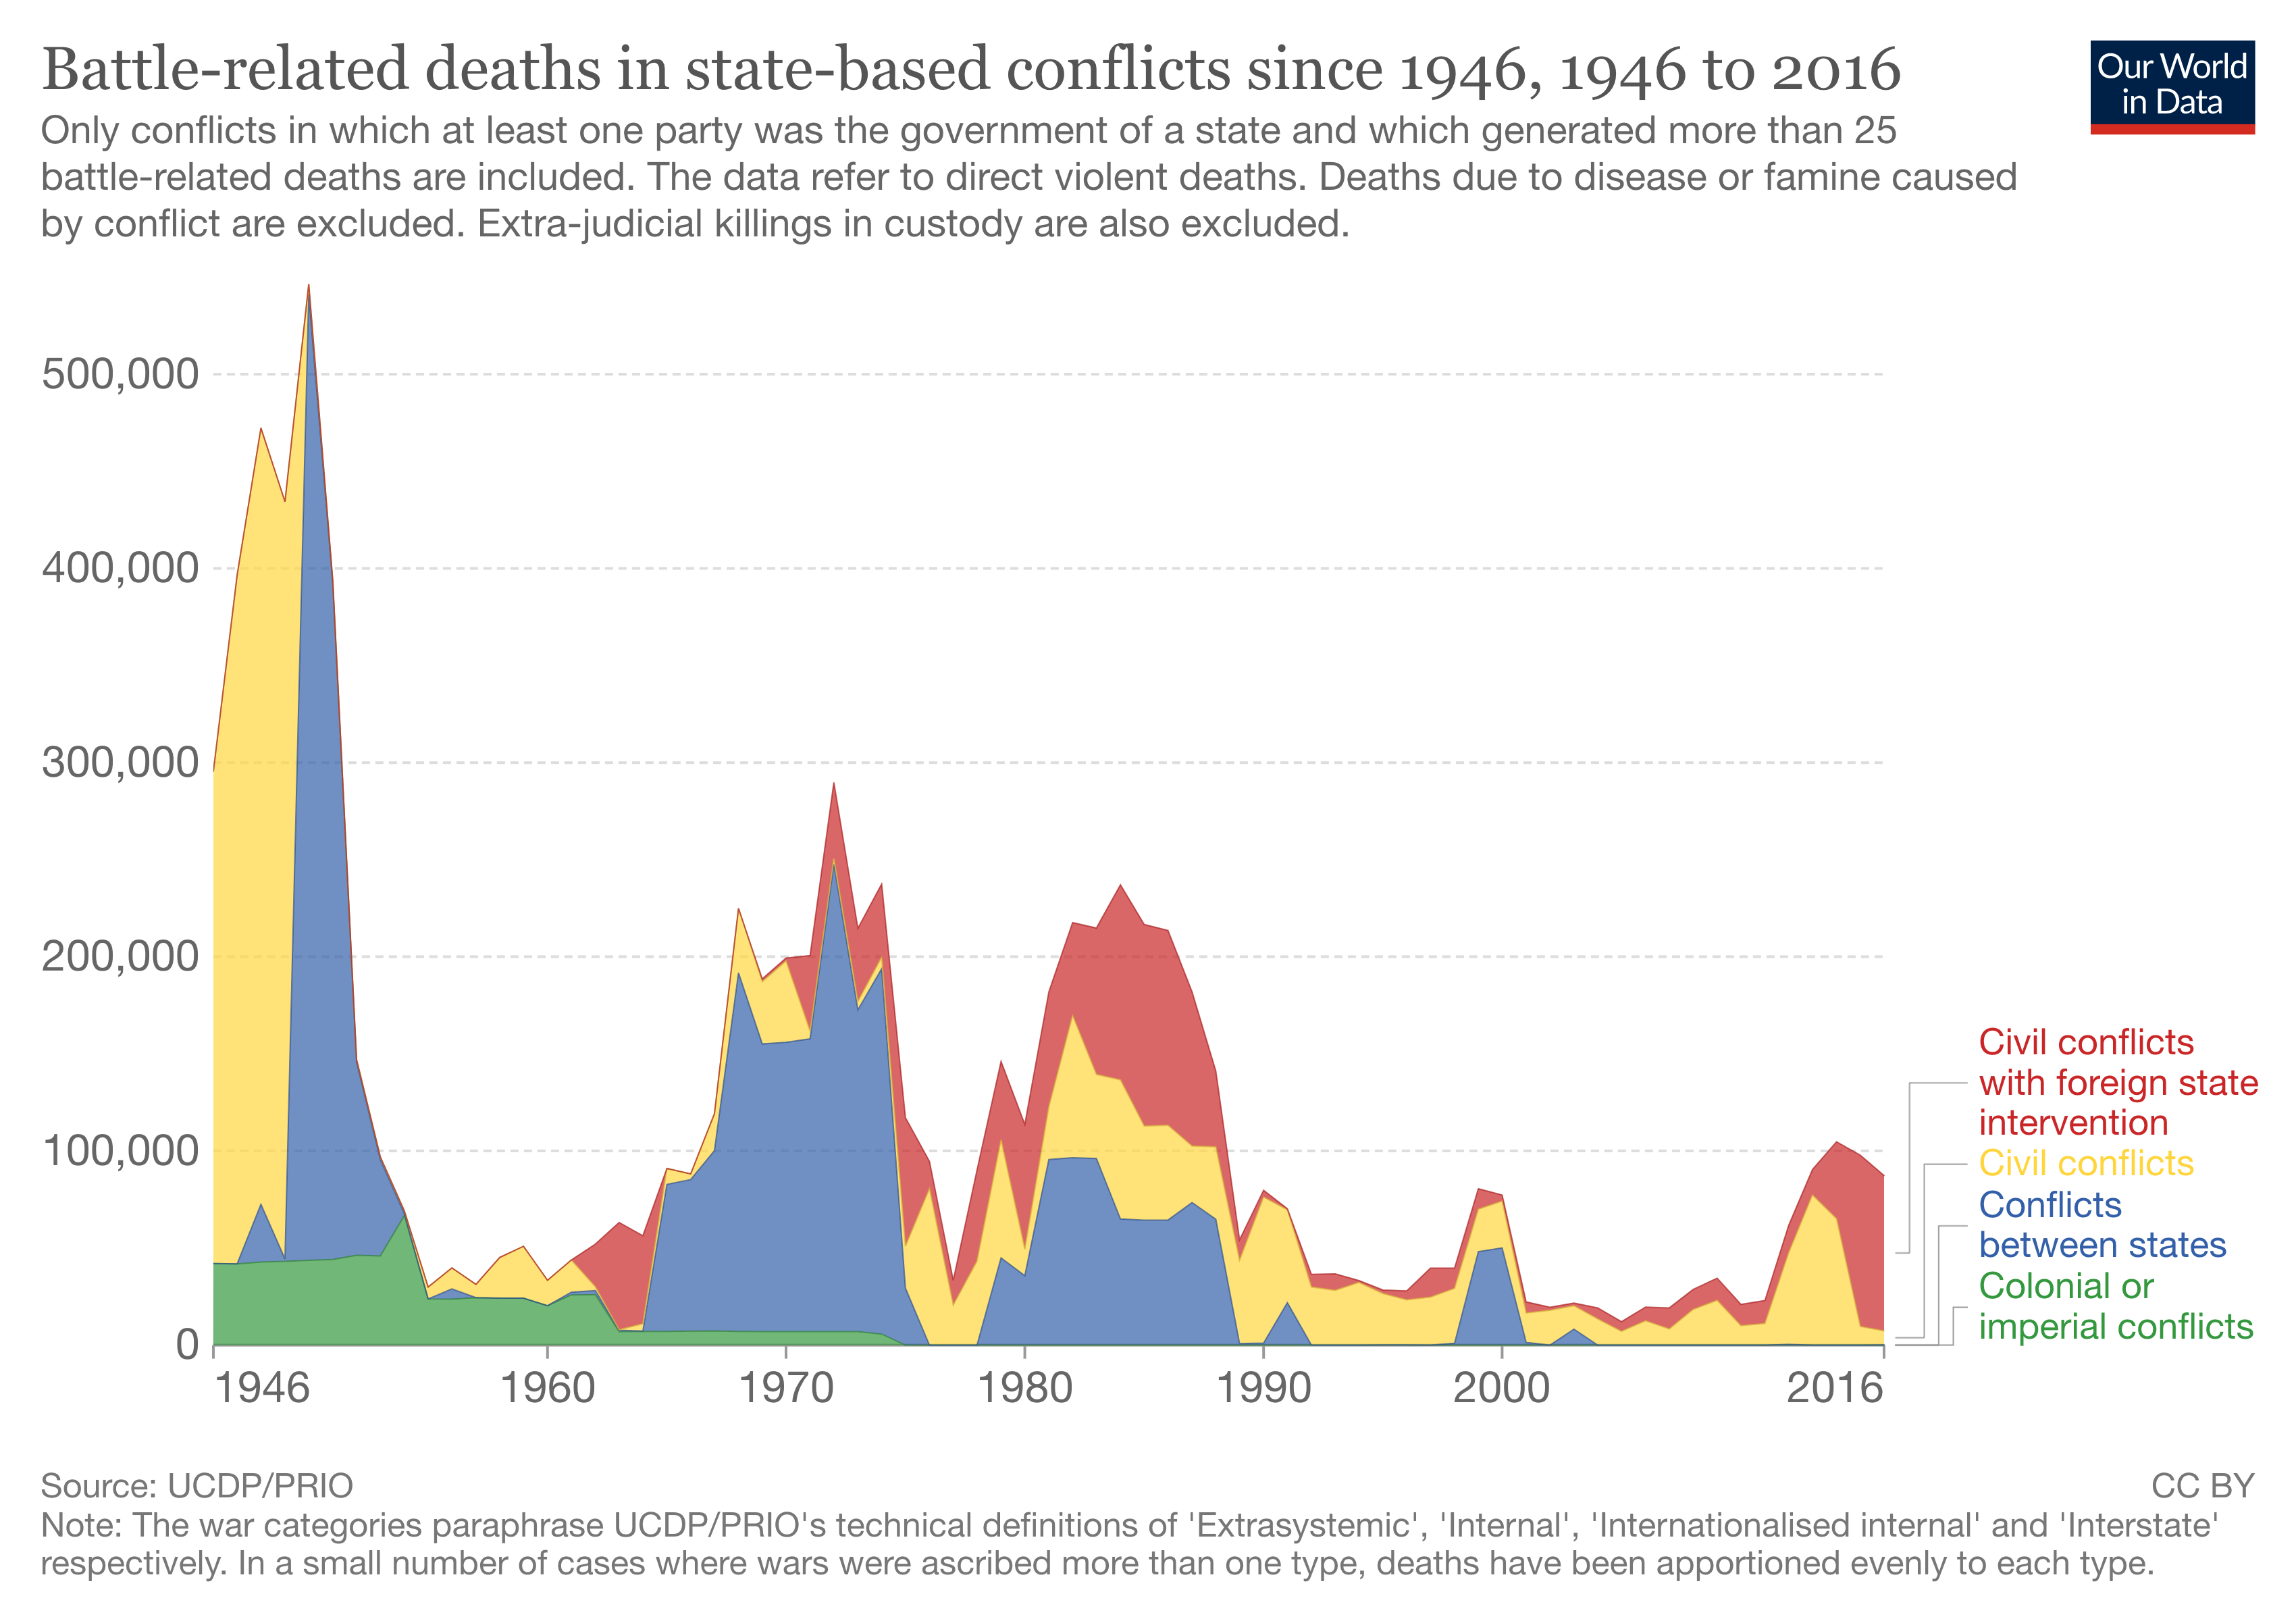
\includegraphics[keepaspectratio, width=\paperwidth, height=.95\paperheight]{../img/battledeaths}};
  \end{tikzpicture}
\end{frame}
% ----------------------------------------------------
\note{Same question, different measure: battle deaths since 1946, UCDP. Read the subtitle aloud: only conflicts with a state as one side, above 25 deaths, direct violent deaths only. Famine and disease excluded.

Now the denominator question: these are absolute counts, and world population roughly tripled over the period. Per capita, the decline looks much steeper. Should it be per capita? It depends on the question: risk to an individual, or the scale of the phenomenon.

And a coverage question: the civil-war share grows over time. Are there more civil wars, or better recording of them?

Three measurement choices, each defensible, each changes the headline.}

% ----------------------------------------------------
\begin{frame}
\frametitle{Description at scale: social capital}
\centering

\begin{itemize}
  \item 21 billion Facebook friendships, 72 million US users aged 25--44
  \vspace{6pt}
  \item Concept: \textbf{economic connectedness}
  \begin{itemize}
    \item share of friends with high socioeconomic status among people with low SES
  \end{itemize}
  \vspace{6pt}
  \item<2-> Mapped by ZIP code, county, high school, college
  \vspace{6pt}
  \item<3-> Among the strongest predictors of upward income mobility they found
\end{itemize}

\vspace{8pt}
{\footnotesize \asher{Chetty et al.\ (2022), Social capital I, \textit{Nature} 608.}}

% TODO: source one Opportunity Insights economic-connectedness map (county level), save as ../img/chetty_ec_map.png
\end{frame}
% ----------------------------------------------------
\note{Mentioned in week 1 as the anchor example for ``describe''. Now properly.

The project is fundamentally a measurement exercise: take a concept (social capital, which sociologists have argued about for decades), split it into dimensions, and build a measure for each from a found dataset. The atlas is public and they can explore it (socialcapital.org).

The third bullet is where it stops being ``only'' description: once you have a good measure, it immediately becomes the input to explanatory questions. Good description is the foundation, not the preliminary.}

% ----------------------------------------------------
\begin{frame}
\frametitle{The design decisions behind the map}
\centering

\begin{itemize}[<+->]
  \item \textbf{Population}: Facebook users aged 25--44. Who is not there?
  \vspace{6pt}
  \item \textbf{SES}: not observed. \textbf{Predicted} from many signals by a model
  \begin{itemize}
    \item a model output, used as a variable. Validated against external data
  \end{itemize}
  \vspace{6pt}
  \item \textbf{Denominator}: share of friends, not number of friends
  \vspace{6pt}
  \item \textbf{Access}: nobody else can rebuild it from the raw data
  \begin{itemize}
    \item released only as aggregates, with noise added for privacy
  \end{itemize}
\end{itemize}

\end{frame}
% ----------------------------------------------------
\note{Everything from today, and most of last week, in one project.

\begin{itemize}
  \item Population: the age band was chosen because Facebook coverage is highest there, a design decision to make the found data as close to representative as possible. Last week's lesson in action.
  \item SES predicted by a model: exactly the classifier-output problem from before the break. They validated it against external income data. That is what doing it properly looks like.
  \item Denominator: share, because the number of friends varies hugely and is itself related to SES.
  \item Access: the post-API point from last week. It is a public good built on private data, and reproducibility depends on trusting the aggregates.
\end{itemize}

Ask them which decision they would challenge first.}

% ----------------------------------------------------
\begin{frame}
\frametitle{Culturomics}
\centering

\begin{itemize}
  \item Google Books: millions of digitised books, word frequencies by year
  \vspace{6pt}
  \item ``Quantitative analysis of culture'': fame, censorship, the spread of ideas
  \vspace{6pt}
  \item<2-> e.g.\ the use of scientific terms rises steadily through the 20th century
  \vspace{6pt}
  \item<3-> Is that a fact about \textbf{culture}, or about \textbf{the corpus}?
\end{itemize}

\vspace{8pt}
{\footnotesize \asher{Michel et al.\ (2011), \textit{Science} 331.}}

% TODO: source an n-gram trend (e.g. from books.google.com/ngrams) and the corpus-composition figure from Pechenick et al. (2015), save as ../img/culturomics_ngram.png and ../img/pechenick_corpus.png
\end{frame}
% ----------------------------------------------------
\note{A large and influential descriptive project: millions of books, word frequencies over centuries, claims about how culture changes. Let them enjoy it for a moment; it is genuinely interesting.

Then the last bullet. Wait for answers before turning the page.}

% ----------------------------------------------------
\begin{frame}
\frametitle{What was actually measured}
\centering

\begin{itemize}[<+->]
  \item The corpus is a \textbf{library}, not a record of what people read
  \begin{itemize}
    \item one copy per book, whether it sold ten copies or ten million
  \end{itemize}
  \vspace{8pt}
  \item Its composition \textbf{changes over time}
  \begin{itemize}
    \item scientific publishing takes up a growing share through the 20th century
  \end{itemize}
  \vspace{8pt}
  \item So a trend in words is partly a trend in \textbf{what got published and digitised}
\end{itemize}

\vspace{10pt}
\uncover<3->{{\footnotesize \asher{Pechenick, Danforth \& Dodds (2015), \textit{PLoS ONE} 10(10).}}}

\end{frame}
% ----------------------------------------------------
\note{Corpus composition is a measurement problem, and it is drift from last week in a different form: the instrument (the corpus) changed composition over the period you are describing.

The first point is the denominator question again: a book is the unit, but culture is about readers. The rise of scientific vocabulary is partly the rise of scientific publishing inside the corpus.

Transfer to their projects: any corpus of posts, news or speeches has the same issue. Before describing a trend in the text, describe the trend in the corpus: who is producing it, and has that changed?}

% ----------------------------------------------------
\begin{frame}
\frametitle{Describing relationships}
\centering

\begin{itemize}
  \item A relationship: knowing one variable tells you something about another
  \vspace{6pt}
  \item<2-> A friend is bringing two kids in your small car. You ask:
  \begin{itemize}
    \item<2-> ``How old are they?'' ``6 and 2.'' Now you know something about size
    \item<3-> ``What colour is their hair?'' You learn nothing about size
  \end{itemize}
  \vspace{6pt}
  \item<4-> That is all a statistical relationship is: \textbf{conditional} values
\end{itemize}

\end{frame}
% ----------------------------------------------------
\note{The intuition in one example, no notation. Age is informative about size; hair colour is not. That is dependence.

It sets up the handover to next week: age does cause size, but the relationship would be just as informative if it did not. The rooster crowing tells you it is morning, and it does not cause the sun to rise.}

% ----------------------------------------------------
\begin{frame}
\frametitle{Describing relationships}
\centering

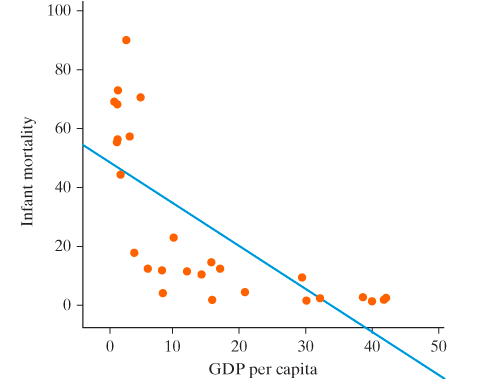
\includegraphics[keepaspectratio, width=0.75\textwidth, height=0.6\paperheight]{../img/scatter_GDP_mort}

\uncover<2->{{\small Infant mortality at \$1{,}000 GDP per capita? At \$30{,}000?}}

\end{frame}
% ----------------------------------------------------
\note{Read the conditional values off the plot: that is the whole of describing a relationship, and it is all statistics does, however complicated it gets.

Then ask: does this tell us that growth reduces infant mortality? It is consistent with that, and with health improving growth, and with institutions driving both. The plot cannot choose between them.

That is the question for next week.}

% ====================================================
\section{Synthesis: wartime civilian deaths}
% ====================================================

% ----------------------------------------------------
\begin{frame}[plain]
  \begin{tikzpicture}[remember picture, overlay]
    \node[at = (current page.center), yshift = 0cm] (cover) {%
      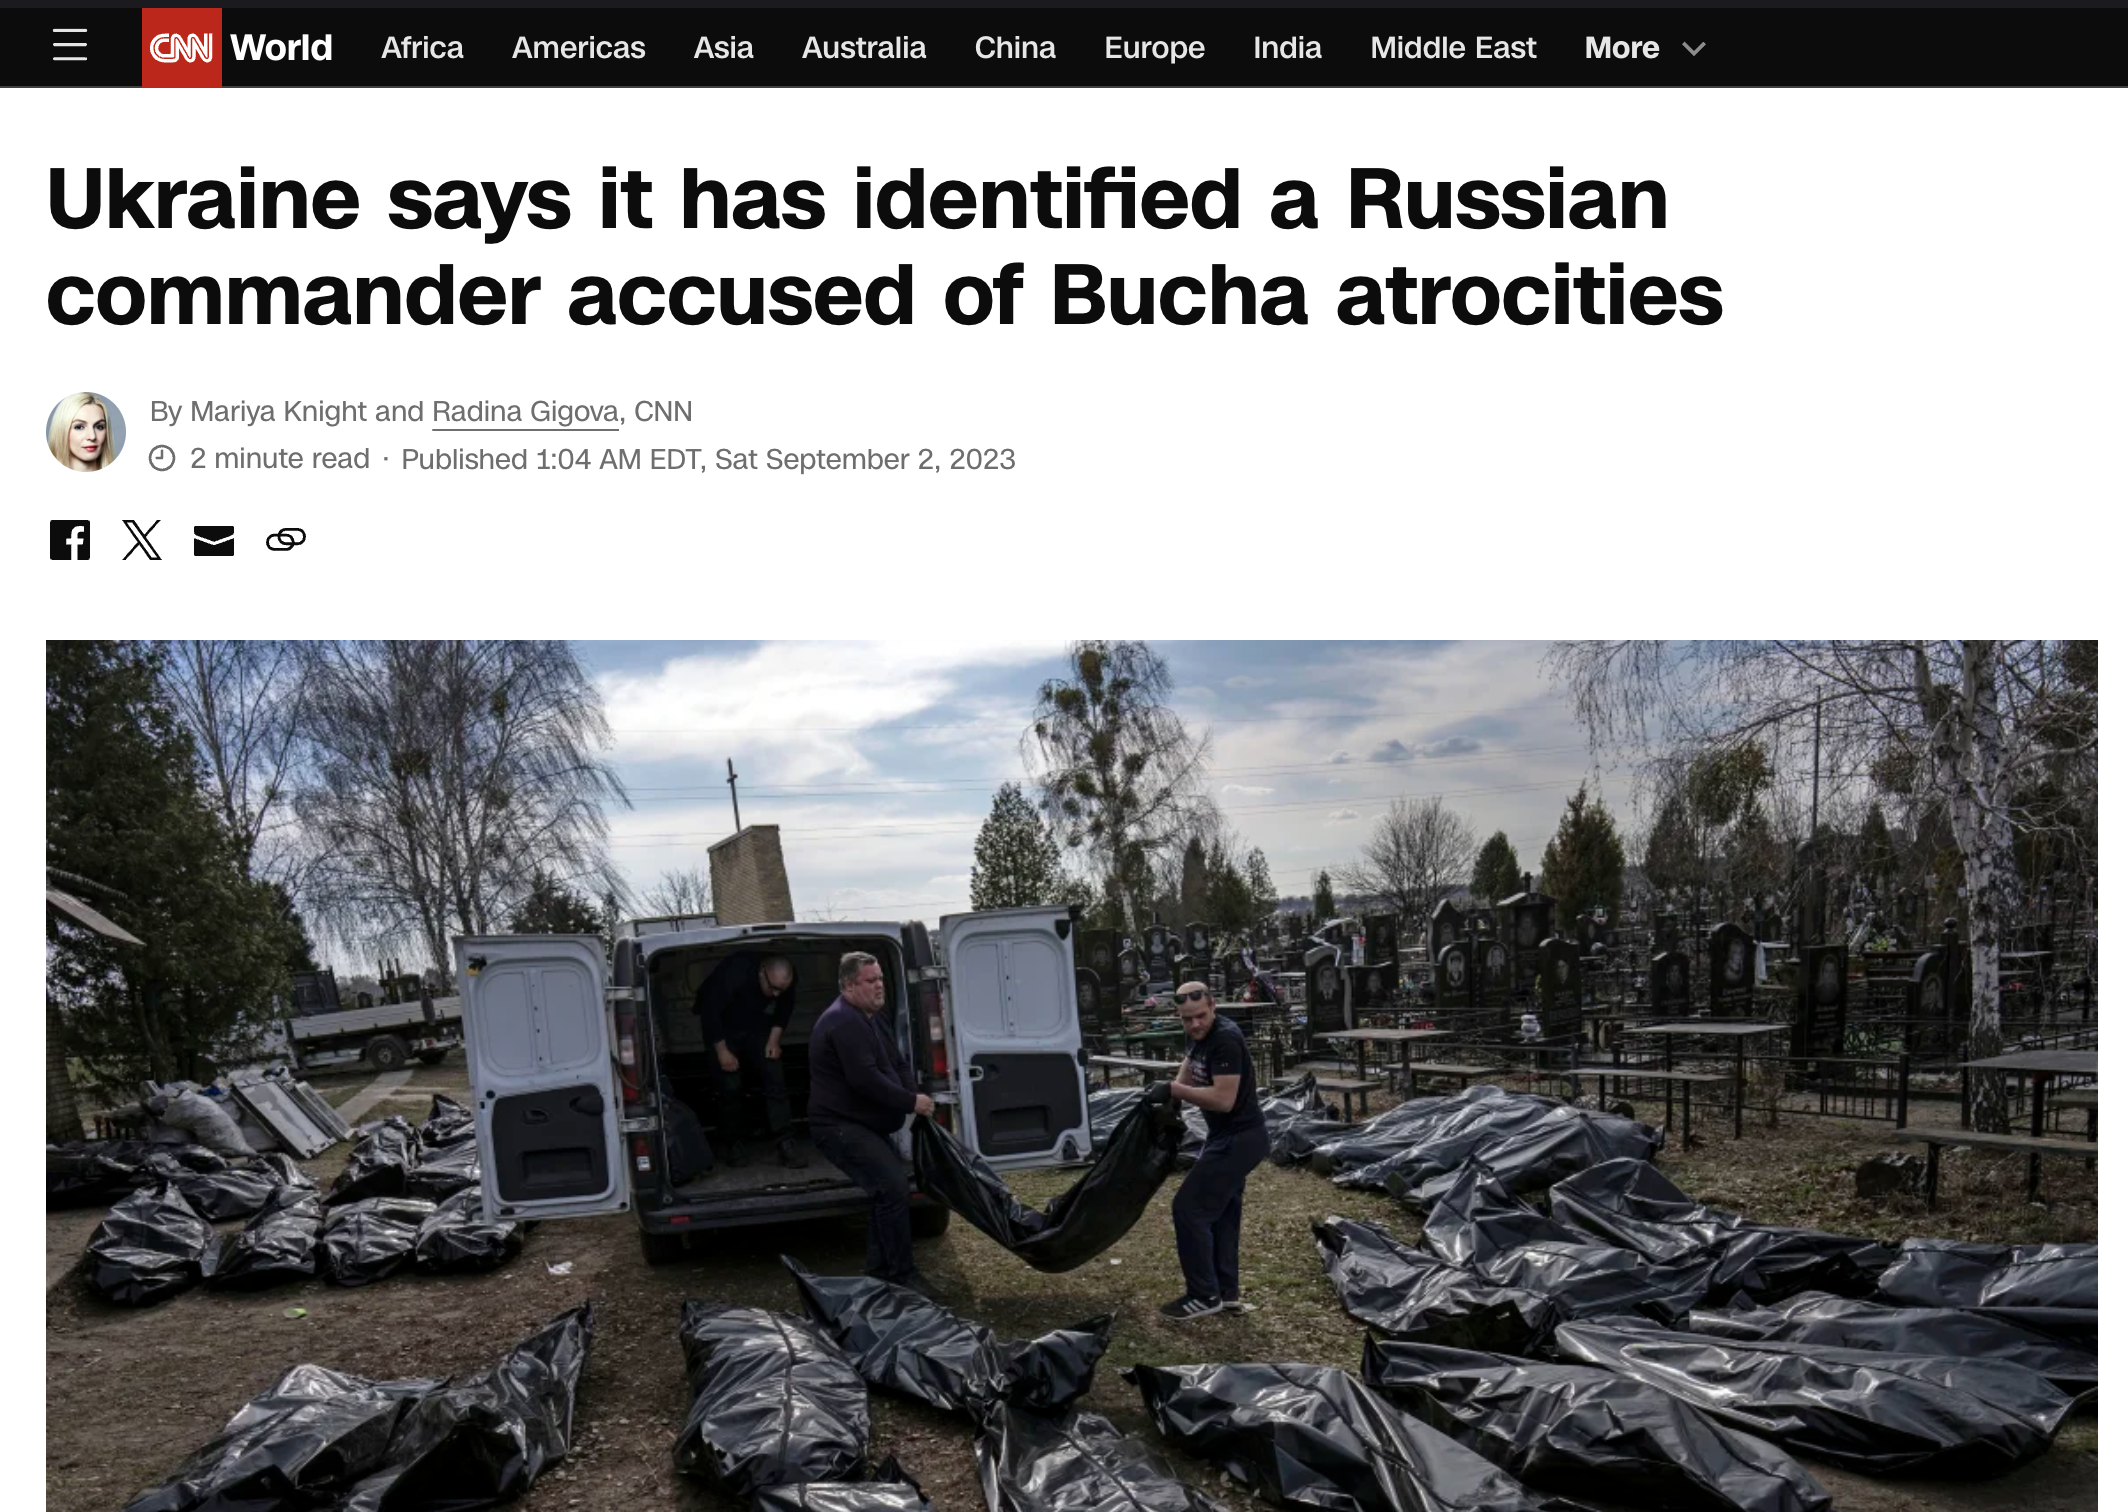
\includegraphics[keepaspectratio, width=\paperwidth, height=\paperheight]{../img/bucha}};
  \end{tikzpicture}
\end{frame}
% ----------------------------------------------------
\note{Bucha, 2022. Say little. Let the image set up the exercise: why do armed groups kill civilians in some places and not others?}

% ----------------------------------------------------
\begin{frame}
\frametitle{Groups of four}
\centering

\begin{itemize}
  \item Intuition: armed groups treat civilians better when they \textbf{need their resources} (labour, food, information) to survive
  \vspace{8pt}
  \item[1.] Clean up the theory. What are the main \textbf{concepts}?
  \item[2.] How would you \textbf{operationalize} them? What would you measure?
  \item[3.] At which \textbf{level}? Who would be \textbf{missing}?
  \item[4.] What \textbf{descriptive} finding would already be worth knowing?
\end{itemize}

\end{frame}
% ----------------------------------------------------
\note{Fifteen minutes, then three groups report. This is the whole session applied end to end, and it is a rehearsal for Memo 3.

What to listen for:
\begin{itemize}
  \item \textbf{Concepts}: ``need'' is the hard one. Local taxation? No external funding? Territorial control?
  \item \textbf{Measures}: event data (UCDP GED, ACLED) is news-based; rural killings are under-reported. Error related to the question, again.
  \item \textbf{Level}: armed group, locality, month?
  \item \textbf{Missing}: places where nobody reported anything.
  \item \textbf{Description}: where violence concentrates is already a contribution.
\end{itemize}

Short of time: ten minutes, two groups.}

% ====================================================
\section{Paper: Roads to Rule, Roads to Rebel}
% ====================================================

% ----------------------------------------------------
\begin{frame}[plain]
  \begin{tikzpicture}[remember picture, overlay]
    \node[at = (current page.center), yshift = 0cm] (cover) {%
      
\includegraphics[keepaspectratio, width=\paperwidth, height=.95\paperheight]{../img/carl1}};
  \end{tikzpicture}
\end{frame}
% ----------------------------------------------------
\note{Müller-Crepon, Hunziker \& Cederman (2021), \textit{JCR}. One minute of summary, then straight to the prompts.

The argument: conflict happens where the state has less reach over a group than the group's own leaders do. That is \textbf{relational} state capacity, and it is the conceptual contribution. The measure: travel times from digitised historical road maps, from the capital to the group (state reach) and within the group (internal cohesion).

Remind them what they were asked to read it for: the concept, and how it becomes a measure.}

% ----------------------------------------------------
\begin{frame}
\frametitle{In pairs/groups}
\centering

\vspace{10pt}
\begin{itemize}
  \item[1.] What is the concept, in one sentence, \textbf{without using the word ``roads''}?
  \vspace{10pt}
  \item[2.] What does the road network \textbf{fail to capture}?
  \vspace{10pt}
  \item[3.] Tell a story where their measure \textbf{goes up} and actual state capacity \textbf{goes down}
\end{itemize}

\end{frame}
% ----------------------------------------------------
\note{Twelve minutes. Prompt 1 on its own, three minutes, take three answers. Then 2 and 3 together.

\begin{itemize}
  \item[1.] The balance between how easily the state reaches a group and how easily the group organises itself. If they need the word roads, they have confused measure and concept, which is the point.
  \item[2.] Radio, phones, air power, local intermediaries, rivers; roads impassable in the rainy season. And roads get built where the state already has capacity.
  \item[3.] A road built to extract resources through hostile territory; roads that help rebels move too; a well-connected region run by a local strongman.
\end{itemize}

Prompt 3 is the most useful: measure and concept can move apart.}

% ----------------------------------------------------
\begin{frame}[plain]
  \begin{tikzpicture}[remember picture, overlay]
    \node[at = (current page.center), yshift = 0cm] (cover) {%
      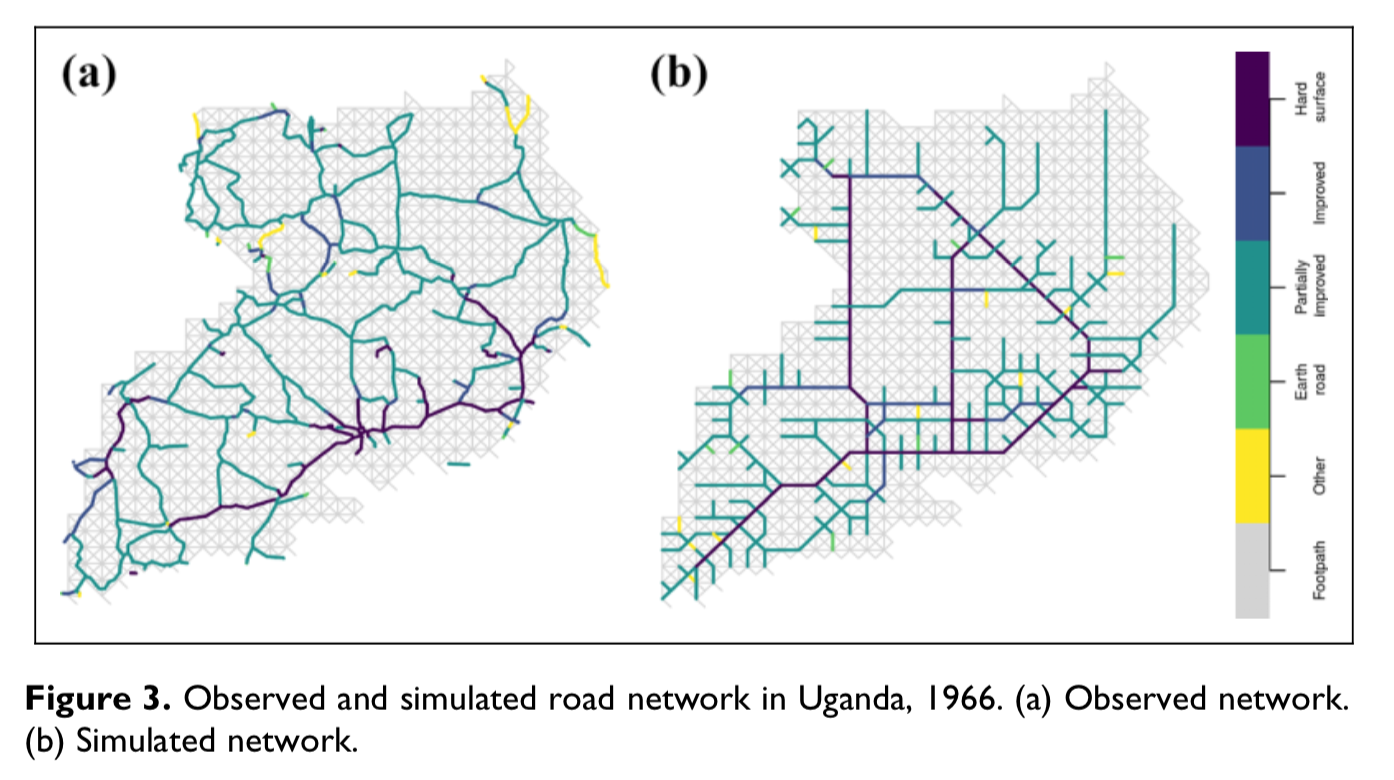
\includegraphics[keepaspectratio, width=\paperwidth, height=.85\paperheight]{../img/carl10}};
  \end{tikzpicture}
\end{frame}
% ----------------------------------------------------
\note{A teaser, one minute. The observed road network in Uganda (left), and a network \textit{simulated} from population distribution alone (right).

Why would they do this? Because roads are not built randomly: the state builds them where it wants control, which is related to conflict risk. The simulated network keeps the part of road-building that comes from where people live, and drops the part that comes from political choices.

That is a causal-design move, and it is week 5. Today, just note that the authors knew their measure was contaminated by the outcome, and designed around it.}

% ----------------------------------------------------
\begin{frame}
\frametitle{Groups of four: build it today}
\centering

\vspace{20pt}
{\large You want to measure relational state capacity\\in 2026, not in 1966.}

\vspace{15pt}
{\large What data would you use, and what would it miss?}

\end{frame}
% ----------------------------------------------------
\note{Seven minutes. Same move as the Google Flu redesign last week: asking what they would build produces engagement where asking them to evaluate produces deference.

Good answers: OpenStreetMap (but volunteer-mapped, so coverage follows where mappers are); mobile coverage and phone records (Blumenstock again); night lights; satellite imagery of roads; administrative presence, such as schools, police stations and courts.

Push each answer through the day's questions: does it capture the concept, is the error related to conflict, who is missing? OSM is a lovely case: it is better mapped where international NGOs have worked, which is often where there has been conflict.}

% ====================================================
\section{Before next week}
% ====================================================

% ----------------------------------------------------
\begin{frame}
\frametitle{The three goals, after today}
\centering

\vspace{10pt}
\begin{itemize}
  \item \textbf{Describe}: measurement \textit{is} the design
  \vspace{8pt}
  \item \textbf{Explain}: a biased measure can manufacture an effect
  \vspace{8pt}
  \item \textbf{Predict}: an accurate prediction of the wrong thing is still wrong
\end{itemize}

\end{frame}
% ----------------------------------------------------
\note{One line per goal, and each has an example from today: Chetty and culturomics for description, the discrimination data for explanation, Obermeyer for prediction.

Close the loop on the opener: Google Flu was an accurate prediction of the wrong thing.}

% ----------------------------------------------------
\begin{frame}
\frametitle{Next week}
\centering

\vspace{25pt}
{\large We can describe a relationship.\\[6pt] Next week: when does it tell us that one thing \textbf{causes} another?}

\end{frame}
% ----------------------------------------------------
\note{Hand over to week 4 with the infant mortality plot in mind: the relationship is real, and it does not tell us why.}

% ----------------------------------------------------
\begin{frame}
\frametitle{Before next week}
\centering

\vspace{8pt}
\begin{itemize}
  \item \textbf{Read:} Guess \textit{et al.}\ (2023), \href{https://www.science.org/doi/10.1126/science.abp9364}{\textit{How do social media feed algorithms affect attitudes and behavior in an election campaign?}}
  \begin{itemize}
    \item Skip the statistics. Read for \textbf{what was randomized}, and \textbf{who took part}
  \end{itemize}
  \vspace{12pt}
  \item<2-> \textbf{Memo 3}, in pairs, Aula Global by \textbf{Monday night}:
  \begin{itemize}
    \item<2-> Pick one concept (not democracy)
    \item<2-> Operationalize it two different ways, with data that exists
    \item<2-> Which would you choose, and what do you lose?
    \item<2-> Half a page
  \end{itemize}
\end{itemize}

\end{frame}
% ----------------------------------------------------
\note{Memo 3 is the first half of today applied to something they choose. ``Not democracy'' because we did it; anything else is fine: polarization, trust, inequality, political interest, misinformation exposure.

Push for two operationalizations that are genuinely different, ideally one designed and one found (a survey item and a behavioural trace), because that is where the interesting trade-offs are. And ask them to say what \textit{each} one would miss.

On the reading: tell them exactly what to read it for. It is a Science paper with a lot of statistics they can skip entirely; the design is in the first two pages.}

% ----------------------------------------------------
\begin{frame}
\frametitle{}
\centering

\vspace{40pt}
{\Large Questions?}

\end{frame}
% ----------------------------------------------------
\note{}
